%% Submissions for peer-review must enable line-numbering 
%% using the lineno option in the \documentclass command.
%%
%% Preprints and camera-ready submissions do not need 
%% line numbers, and should have this option removed.
%%
%% Please note that the line numbering option requires
%% version 1.1 or newer of the wlpeerj.cls file, and
%% the corresponding author info requires v1.2

%% For a neater looking manuscript (to share with colleagues):
%\documentclass[fleqn,10pt]{wlpeerj} % for preprint submissions
%\newcommand{\n}[1]{{\color{black}#1}}

% For review:
\documentclass[fleqn,10pt,lineno]{wlpeerj} % for journal submissions
%\newcommand{\n}[1]{{\color{blue}#1}} % color modified text blue 
\newcommand{\n}[1]{{\color{black}#1}} % color modified text back (normal)

\usepackage{bbding} %for FiveStarOpen
\usepackage{changepage} % for adjustwidth
\usepackage{amssymb}
\usepackage{amsmath}
\usepackage{upgreek}
\usepackage[]{fontenc}
\usepackage{color}
\usepackage{bm}
\usepackage[english]{babel}
\usepackage{graphicx}
\usepackage{tikz}
\usetikzlibrary{positioning}
\usepackage{ifthen}
\usepackage{xstring}
\usepackage{afterpage}
%\usepackage[hidelinks]{hyperref}
%\usepackage[colorlinks=true, allcolors=blue, pdfborder={0 0 0}]{hyperref}
\usepackage[colorlinks=false, allcolors=blue, pdfborder={0 0 0}]{hyperref}

\newcommand{\floor}[1]{\left \lfloor #1 \right \rfloor}
\newcommand{\round}[1]{\left \lfloor #1 \right \rceil }
\newcommand{\ceil}[1]{\left \lceil #1 \right \rceil }
\newcommand{\Fig}[1]{Fig.~\ref{#1}}
%\newcommand{\Fig}[1]{Figure~\ref{#1}}
\newcommand{\Figs}[1]{Figs.~\ref{#1}}
%\newcommand{\Figs}[1]{Figures~\ref{#1}}
\newcommand{\Sec}[1]{Section~\ref{#1}}
\newcommand{\Secs}[1]{Sections~\ref{#1}}
\newcommand{\Chap}[1]{Chapter~\ref{#1}}
\newcommand{\Chaps}[1]{Chapters~\ref{#1}}
\newcommand{\Tab}[1]{Table~\ref{#1}}
\newcommand{\Tabs}[1]{Tables~\ref{#1}}
\newcommand{\Eqn}[1]{Eqn.~\ref{#1}}
\newcommand{\Eqns}[1]{Eqns.~\ref{#1}}
\newcommand{\InEqn}[1]{Inequality~(\ref{#1})}
\newcommand{\InEqns}[1]{Inequalities~(\ref{#1})}
\newcommand{\Center}[1]{\textcolor{white}{.}\hfill#1\hfill\textcolor{white}{.}}
\newcommand{\ang}{$\textrm\AA$\xspace}
\newcommand{\new}[1]{#1}
\newcommand{\New}[1]{#1}
\newcommand{\we}{I~}
\newcommand{\h}{h}

\newcommand{\cis}{{\em{cis}}\xspace}
\newcommand{\trans}{{\em{trans}}\xspace}

\newcommand\solidrule[1][1cm]{\rule[0.5ex]{#1}{0.2mm}}
\newcommand\dotdashedrule{\mbox{%
  \solidrule[1.5mm]\hspace{0.75mm}\solidrule[0.2mm]\hspace{0.75mm}\solidrule[1.5mm]}}
\newcommand\dashedrule{\mbox{%
  \solidrule[1.5mm]\hspace{0.75mm}\solidrule[1.5mm]}}
\newcommand\dottedrule{\mbox{%
  \solidrule[0.2mm]\hspace{0.3mm}\solidrule[0.2mm]\hspace{0.3mm}\solidrule[0.2mm]\hspace{0.3mm}\solidrule[0.2mm]\hspace{0.3mm}\solidrule[0.2mm]\hspace{0.3mm}\solidrule[0.2mm]}}
  
  
\usepackage{xspace}

\newcommand{\code}[1]{\texttt{#1}\xspace}

\usepackage[cal=cm,scrscaled=1.05]{mathalfa} % This is for \mathcal{}, particularly \mathcal{R}
\DeclareMathAlphabet\mathbfcal{OMS}{cmsy}{b}{n} % for boldface mathcal: \mathbfcal{}
\newcommand{\rr}{$\mathcal{R}$\xspace}


\def\kt{k_{\rm B}T}


\def\beq{\begin{equation}}
\def\eeq{\end{equation}}
\def\bea{\begin{eqnarray}}
\def\eea{\end{eqnarray}}

\def\cal#1{\mathcal{#1}}
\def\eqq#1{Eq.~(\ref{#1})}
\def\eq#1{(\ref{#1})}
\def\av#1{\langle #1 \rangle}

\def\f#1{Fig.~\ref{#1}}
\def\ff#1{Figs.~\ref{#1}}

\def\s#1{Section~\ref{#1}}

\def\c#1{~\cite{#1}}


%\newcommand{\c}[1]{\citep{#1}}

%\title{On the other hand: a survey of peptide backbone twist using a new metric for `handedness' ($\bm\h$)}
\title{An exhaustive survey of regular peptide conformations using a new metric for backbone handedness ($\bm\h$)}

\author[1,2,*]{Ranjan V. Mannige}
%\author[1]{Other Names TBD}
\affil[1]{~Molecular Foundry, Lawrence Berkeley National Laboratory, Berkeley, CA, U.S.A.}
\affil[2]{~Present address: Multiscale Institute, Redwood City, CA, U.S.A.}
\affil[*]{~ranjanmannige@gmail.com}

% \keywords{Protein structure, Backbone Chirality, Backbone Twist}

\begin{abstract}
%Proteins are a class of biomolecules that display diverse conformations, which is the reason for their diverse functionality. These conformations are afforded in large part due to a protein's backbone, whose twists and contortions allow for a protein to fold into particular conformations. 
The Ramachandran plot is important to structural biology as it describes a peptide backbone in the context of its dominant degrees of freedom -- the backbone dihedral angles $\phi$ and $\psi$ \citep{Ramachandran1963}. Since its introduction, the Ramachandran plot has been a crucial tool to characterize protein backbone features. However, the conformation or twist of a backbone as a function of $\phi$ and $\psi$ has not been completely described for both \cis and \trans backbones. Additionally, little intuitive understanding is available about a peptide's conformation simply from knowing the $\phi$ and $\psi$ values of a peptide (e.g., is the regular peptide defined by $\phi=\psi=-100^\circ$ left-handed or right-handed?). 
This report provides a new metric for backbone handedness ($\h$) based on interpreting a peptide backbone as a helix with axial displacement $d$ and angular displacement $\theta$, both of which are derived from a peptide backbone's internal coordinates, especially dihedral angles $\phi$, $\psi$ and $\omega$. In particular, $\h$ \n{equals} $\sin(\theta)d/|d|$, with range $[-1,1]$ and negative (or positive) values indicating left(or right)-handedness. The metric $\h$ is used to characterize the handedness of every region of the Ramachandran plot for both \cis ($\omega=0^\circ$) and \trans ($\omega=180^\circ$) backbones, which provides the first exhaustive survey of twist handedness in Ramachandran $(\phi,\psi)$ space. These maps fill in the `dead space' within the Ramachandran plot, which are regions that are not commonly accessed by structured proteins, but which may be accessible to intrinsically disordered proteins, short peptide fragments, and protein mimics such as peptoids. 
Finally, building on the work of \cite{Zacharias2013}, this report presents a new plot based on $d$ and $\theta$ that serves as a universal and intuitive alternative to the Ramachandran plot. The universality arises from the fact that the co-inhabitants of such a plot include every possible peptide backbone including \cis and \trans backbones. The intuitiveness arises from the fact that $d$ and $\theta$ provide, at a glance, numerous aspects of the backbone including compactness, handedness, and planarity. 
\end{abstract}


\begin{document}

\flushbottom
\maketitle
\thispagestyle{empty}

\section*{Introduction}

% Protein intro: backbone conformation is important
The backbone of a protein (\Fig{fig:intro}a) can twist and turn into numerous conformations (folds), in part due to the amino acid sequence that the protein displays. %It is partly for this reason that, as a class of biomolecules, proteins are unparalleled in the diversity of their functionality \citep{Alberts2002,Berg2006}. 
Understanding how a backbone twists is of great importance to the field of biochemistry, since understanding the structure of a protein goes a long way towards understanding how a protein functions \citep{Alberts2002,Berg2006}. While the conformation of a peptide backbone is dependent on a number of parameters (bond lengths, bond angles, and dihedral angles), \cite{Ramachandran1963} recognized that the twist of a peptide backbone can be described to a great degree by the dihedral angles $\phi$ and $\psi$ (\Fig{fig:intro}a).

% Backbone intro, ramachandran plot intro.
Today, two-dimensional $(\phi,\psi)$ plots are called Ramachandran plots (or `maps'), and are introduced in undergraduate biology textbooks as a guide for understanding a peptide backbone's general conformational state or `twistedness' at a glance 
\citep{Bragg1950, Pauling1951a, Pauling1951, Linderstrom-Lang1952, Laskowski1993, Chothia1997, Hooft1997, Cooper2000, Alberts2002, Laskowski2003, Ho2003, Eisenberg2003, Berg2006, Mannige2016}. 
The Ramachandran plot is especially useful because (stable) proteins are hierarchical in structure \citep{Linderstrom-Lang1952}: the final (tertiary) conformation of a {\em structured} protein is composed of discrete secondary structures -- {\em regular} structures -- that interact with each other and \n{which} are strung together by loops that are less regular \citep{Alberts2002,Berg2006}. Each regular \n{peptide} structure describes a backbone whose per-residue $(\phi,\psi)$ values are generally the same, and therefore their `locations' on the Ramachandran plot act as structural landmarks (\Fig{fig:intro}b).
%These secondary structures pack together into globular conformations (tertiary structures) with the help of loops, which are also specifically twisted due to their $\phi$ and $\psi$ angles \citep{Berg2006}.}
%Any peptide built with uniform twist or backbone parameters (say, $\phi=X^\circ$ and $\psi=Y^\circ$) will result in a regular structure; some regular structures are energetically stable (or metastable) and are called secondary structures (\Fig{fig:intro}b). These secondary structures often pack together into globular structures with the help of loops, which are also twisted \citep{Berg2006}. 

\begin{figure}[t!]
\centering
\includegraphics[width=0.8\linewidth]{./figures/chirality_intro.pdf}
\caption{\label{fig:intro} 
The backbone of a single residue (a) can be described by its dihedral angles $\phi$ and $\psi$ (and in smaller part, $\omega$, which is predominantly \trans or $\sim 180^\circ$). \n{The Ramachandran plot is important because a number of regular conformations important to biology -- secondary structures -- are located at specific regions of the plot (b). For the most part, regular peptide backbones twist in either a left-handed or right-handed fashion}; examples are shown in (c). 
As evidenced in (b), the -ve diagonal within the Ramachandran plot (dashed line described by \n{$\phi=-\psi$}) divides right-handed peptides from left-handed peptides, which leads to the na{\"i}ve picture of handedness (d). \cite{Zacharias2013} showed that this picture is over simplistic, however an in-depth characterization of the backbone in all regions was not performed, and will be done here for both \cis ($\omega=0$) and \trans backbones ($\omega=\uppi$). Panel (a) is modified from \cite{Mannige2016}. Due to low \n{incidence} within the studied database (see Methods), the two left-handed helices in (b) are arbitrarily marked and have no statistical significance. \n{A}ll molecular representations in this text are shown in `licorice' form, with the colors red, blue and white representing oxygen, nitrogen and carbon atoms. 
}
\end{figure}

% Limitations: only structured proteins are well characterized today, even though there are many other types of proteins and protein-like molecules out there.
So far, our understanding of the Ramachandran plot has been limited mostly to structured proteins that display stable conformations \citep{Berman2000,Alberts2002}. These types of proteins occupy only a limited region of the plot (dotted regions in \Fig{fig:intro}b). The regular backbone conformations in these regions are well understood\n{. F}or example, known regular structures that are to the right of the negatively sloping diagonal (dashed line in \Fig{fig:intro}b; henceforth denoted as the `-ve diagonal') are left-handed in backbone twist, while those that are to the left of the diagonal are right-handed (left- and right-handed regions are respectively shaded brown and gold\footnote{Go Hillies!}). For example, the position of the idealized left- and right-handed $\upalpha$-helices (\Fig{fig:intro}c) -- respectively denoted as $\upalpha_\textrm{L}$ and $\upalpha$ in \Fig{fig:intro}b -- are on opposite sides of the -ve diagonal. The `na{\"i}ve view' of handedness, obtained from looking only at structured proteins, would be the expectation that the -ve diagonal neatly separates the Ramachandran plot into regions of left- and right-handedness (\Fig{fig:intro}d).

However, structured proteins represent only a fraction of functional proteins. Indeed, up to 15\% of mammalian proteins are completely disordered -- they natively display multiple, often extended, conformations -- and up to 50\% of the mammalian proteins display large ($>30$ residue) stretches of disorder \citep{Iakoucheva2002,Ward2004,Orosz2011,Mannige2014b}. Interestingly, when compared to structured backbones, structurally degenerate or disordered backbones occupy many more regions within the Ramachandran plot \citep{Beck2008}.

Additionally, a number of peptide mimics -- especially peptoids \citep{Sun2013} -- \n{have been found to} display novel secondary structures that occupy regions that are strictly disallowed by proteins due to steric clashes. %For example, peptide mimics  called pep\textit{toids} \citep{Sun2013} display new secondary structures that fall out of the regions regularly occupied by proteins \citep{Sun2013,Goodman2007,Culf2010,Beke2006,Pohl2012,Zuckermann2009,Sun2013}. %This is possible because of the `subtle' chemical differences between peptides and peptoids: peptoids are distinguished from peptides by the position of each sidechain on the backbone [sidechains are attached to the backbone nitrogen atom rather than the $\upalpha$-carbon; \cite{Sun2013}]. 
For example, a `higher-order' peptoid secondary structure -- the $\Sigma$-strand \citep{Mannige2015,Robertson2016} -- \n{is believed to sample} regions of the Ramachandran plot (`$\textrm{\textbf{I}}$' in \Fig{fig:intro}b) that are not permitted within natural proteins (\n{this is because peptoid backbones lack hydrogen-bond donors}). Another \n{peptoid} secondary structure -- the `$\omega$-strand' \citep{Gorske2016} -- samples similarly historically uncharted regions of the Ramachandran plot (`$\textrm{\textbf{II}}$' in \Fig{fig:intro}b). Importantly, backbone twist handedness plays a crucial part in explaining these new motifs: as one goes along the backbones of these secondary structures, alternating residues 
\n{display backbone twists that are equal in magnitude but opposite in handedness} [for this reason, the $\Sigma$-strand is relatively linear, albeit meandering; \cite{Mannige2015}; \cite{Mannige2016}].

Despite these recent discoveries of natively disordered proteins and novel peptidomimetic structures, a complete understanding of backbone conformations that stray from the `structured' regions on the Ramachandran plot is missing, which impedes our ability to identify and explore such conformations. Towards filling this gap in understanding, this report outlines a detailed study of how regular backbones twist in every region of the Ramachandran plot \n{for both \cis and \trans peptides}. In particular, this report develops and explores a new metric for handedness ($\h$) based on modeling a regular backbone (described below) as a helix \citep{Shimanouchi1955,Miyazawa1961,Zacharias2013}. The metric is used to exhaustively chart the handedness of regular backbones. In doing so, this survey provides a new graphical format to explore new types of secondary structures being discovered \citep{Mannige2015,Gorske2016}\n{. Also, this survey dispels} the na{\"i}ve view of handedness (\Fig{fig:intro}d) by showing that the distribution of handedness as a function of $\phi$ and $\psi$ is more complicated than the distribution allowed by the na{\"i}ve view. Finally, the results also show that the Ramachandran plot whose $\phi$ and $\psi$ values range between $0^\circ$ and $360^\circ$ is more intuitive and visually meaningful (compared to those that range between $-180^\circ$ and $180^\circ$), particularly for \cis backbones. \n{T}his work builds on a previous report \citep{Zacharias2013} and helps complete our understanding of the ways in which a peptide backbone twists, which is a basic component of structural biology.

\section*{Methods}
While angular units in this report switch between radians and degrees, their units in any particular situation may be inferred by the presence or absence of the degree symbol ($^\circ$). All methods and materials required to produce this manuscript are freely available at \url{https://github.com/ranjanmannige/backbone_chirality}.

\subsection*{Deriving measures for backbone handedness}
Numerous metrics for molecular chirality and handedness have so far been discussed \citep{Harris1999}. For example, metrics for chirality have been introduced that focus on vector orientations \citep{Kwiecinska2005,Kabsch1983,Gruziel2013}, optical activity \citep{Osipov1995}, and molecular shape \citep{Ferrarini1998}. However, this report will focus on a simpler metric for chirality associated with an idealized helix within which 
all (regular) backbone atoms of one type sit \n{[\Fig{fig:helix};} \cite{Shimanouchi1955,Miyazawa1961,Zacharias2013}\n{]}. 
%This can be done because any {\em regular} backbone can be associated with a specific helix. %\footnote{Indeed, the word `helix' has a broader meaning that comes from the Greek word $\check\epsilon\lambda\iota\xi$ that means `twisted, curved'; \cite{Liddell1894}.}, 
Here, a `regular' backbone  indicates that each tunable parameter within a unit or `residue' -- say a particular dihedral angle -- remains the same for all residues. Below, regular backbones are modeled in context of helical parameters that, when combined, form an intuitive metric for backbone handedness.

\subsection*{Describing a regular backbone as a helix} 
Interest in how a backbone may be represented as a helix emerged shortly after the first secondary structures were introduced \citep{Pauling1951,Pauling1951a,Pauling1951b}. In particular, \cite{Shimanouchi1955} had derived a set of equations that fit a platonic helix to the atoms within a regular backbone. 
While the formalisms described by \cite{Shimanouchi1955} [and later on by \cite{Miyazawa1961}, discussed below] apply to repeating linear polymers of arbitrary complexity, %[allowing for the treatment of even biomimics that do not conserve atom arrangements \citep{Kandakov2013}), 
this report focuses specifically on how peptides may be modeled. \Fig{fig:helix} describes an arbitrary peptide backbone that may be represented either using internal coordinates \textit{(i)} or helical coordinates \textit{(ii)}. 

\begin{figure}[t!]
\mbox{}\hfill
\includegraphics[width=0.95\textwidth]{./figures/helix_peptide.pdf}
\hfill\mbox{}\hfill\mbox{}\newline
\caption{\label{fig:helix}
Internal coordinate \textit{(i)} and helical coordinate \textit{(ii)} representations of right-handed (a) and left-handed (b) regular backbones. Internal coordinates are a function of bond lengths (e.g., \n{$v_{23}$}), angles ($\sigma_{2}$), and dihedral angles \n{($\tau_{12}$)}, while helical coordinates are a function of displacement along the helical axis ($d_{12}$), angular displacement in the plane perpendicular to the helical axis ($\theta_{12}$) and shortest distance of an atom of type $i$ \n{to} the helical axis ($\rho_i$). Representations are derived from Figs.~1 and~2 in  \cite{Shimanouchi1955}.
}
\end{figure}

Internal coordinates are associated with stereochemical terms: bond lengths ($v_{ij}$) between adjacent atoms $i$ and $j$, bond angles ($\sigma_{i}$) between the two bonds adjacent to atom $i$, and dihedral or torsion angles ($\tau_{ij}$), which involve atoms associated with the bond $i-j$ \n{and the two adjacent atoms}. Helical coordinates (\Fig{fig:helix}\textit{(ii)}) are described using measures of \n{axial} displacement \n{between two successive atoms of the same type} ($d$; this is related to the pitch of a platonic helix), angular displacement \n{between two successive atoms of the same type} ($\theta$), and the radius of the helix ($\rho_i$) that hosts all backbone atoms of type $i$. Therefore, the single cylinder shown in \Fig{fig:helix} is too simplistic as there should be one distinct cylinder or radius per atom type.

Given that there are three \n{backbone} atoms associated with a residue (\Fig{fig:intro}a), $d = d_{\textrm{n},\upalpha}+d_{\upalpha,\textrm{c}}+d_{\textrm{c},\textrm{n}}$ and $\theta = \theta_{\textrm{n},\upalpha}+\theta_{\upalpha,\textrm{c}}+\theta_{\textrm{c},\textrm{n}}$. Here, $d_{i,j}$ and $\theta_{i,j}$ respectively refer to the axial and angular displacement between adjacent atoms $i$ and $j$. Subscripts `$\textrm{n}$', `$\upalpha$', and `$\textrm{c}$' respectively refer to the backbone nitrogen, $\upalpha$-carbon and carbonyl carbon atoms (\Fig{fig:intro}a). The notation used by \cite{Shimanouchi1955} was in terms of matrices, which were then simplified by \cite{Miyazawa1961} into trigonometric terms. In particular, \cite{Miyazawa1961} noted that the total residue-residue \n{axial} displacement ($d$) and angular displacement ($\theta$) may be retrieved using the following two equations.

\begin{align}
\cos\left(\frac{\theta}{2}\right) =&\cos\left(\frac{+\phi+\psi+\omega}{2}\right) \sin\left(\frac{\sigma_\textrm{n}}{2}\right) \sin\left(\frac{\sigma_\upalpha}{2}\right) \sin\left(\frac{\sigma_\textrm{c}}{2}\right) \nonumber \\
                                  -&\cos\left(\frac{+\phi-\psi+\omega}{2}\right) \sin\left(\frac{\sigma_\textrm{n}}{2}\right) \cos\left(\frac{\sigma_\upalpha}{2}\right) \cos\left(\frac{\sigma_\textrm{c}}{2}\right) \nonumber \\
                                  -&\cos\left(\frac{+\phi+\psi-\omega}{2}\right) \cos\left(\frac{\sigma_\textrm{n}}{2}\right) \sin\left(\frac{\sigma_\upalpha}{2}\right) \cos\left(\frac{\sigma_\textrm{c}}{2}\right) \nonumber \\
                                  -&\cos\left(\frac{-\phi+\psi+\omega}{2}\right) \cos\left(\frac{\sigma_\textrm{n}}{2}\right) \cos\left(\frac{\sigma_\upalpha}{2}\right) \sin\left(\frac{\sigma_\textrm{c}}{2}\right)
                                  \label{eqn:theta}
\end{align}
\begin{align} 
d \sin\left(\frac{\theta}{2}\right) = & \left(+v_{\textrm{n,}\upalpha}+v_{\upalpha\textrm{,c}}+v_\textrm{c,n}\right)\sin\left(\frac{+\phi+\psi+\omega}{2}\right)\sin\left(\frac{\sigma_\textrm{n}}{2}\right)\sin\left(\frac{\sigma_\upalpha}{2}\right)\sin\left(\frac{\sigma_\textrm{c}}{2}\right)\nonumber \\
                                    - & \left(+v_{\textrm{n,}\upalpha}-v_{\upalpha\textrm{,c}}+v_\textrm{c,n}\right)\sin\left(\frac{+\phi-\psi+\omega}{2}\right)\sin\left(\frac{\sigma_\textrm{n}}{2}\right)\cos\left(\frac{\sigma_\upalpha}{2}\right)\cos\left(\frac{\sigma_\textrm{c}}{2}\right)\nonumber \\
                                    - & \left(+v_{\textrm{n,}\upalpha}+v_{\upalpha\textrm{,c}}-v_\textrm{c,n}\right)\sin\left(\frac{+\phi+\psi-\omega}{2}\right)\cos\left(\frac{\sigma_\textrm{n}}{2}\right)\sin\left(\frac{\sigma_\upalpha}{2}\right)\cos\left(\frac{\sigma_\textrm{c}}{2}\right)\nonumber \\
                                    - & \left(-v_{\textrm{n,}\upalpha}+v_{\upalpha\textrm{,c}}+v_\textrm{c,n}\right)\sin\left(\frac{-\phi+\psi+\omega}{2}\right)\cos\left(\frac{\sigma_\textrm{n}}{2}\right)\cos\left(\frac{\sigma_\upalpha}{2}\right)\sin\left(\frac{\sigma_\textrm{c}}{2}\right)
                                    \label{eqn:d}
\end{align}
The ranges for $d$ and $\theta$, respectively, are $[-\lambda,+\lambda]$ and $[0,2\uppi)$ (the positive limit $\lambda$ is defined by allowed values for the various internal coordinates). As above, subscripts `$\textrm{n}$', `$\upalpha$', and `$\textrm{c}$' respectively refer to the backbone nitrogen, $\upalpha$-carbon and carbonyl carbon atom \n{types}. %; $v_{ij}$ refers to the distance between adjacent atoms of type $i$ and $j$; $\sigma_i$ refers to the angle between the adjacent \n{backbone} bonds \n{that share an atom of type $i$}. 
The dihedral angles $\phi$, $\psi$, and $\omega$ represent the traditional  symbols for backbone dihedral angles, which may be otherwise denoted as $\tau_{\textrm{n},\upalpha}$, $\tau_{\upalpha,\textrm{c}}$, and $\tau_{\textrm{c},\textrm{n}(+1)}$, respectively. 

Finally, for any type of atom (say $\upalpha$-carbons), the radius or distance from the helical axis $\rho_\upalpha$ is defined by
\begin{align} 
2 \rho_\upalpha^2 \left[1 - \cos(\theta)\right] + d^2 = & ~v_{\upalpha,\textrm{c}}^2 + v_{\textrm{c},\textrm{n}}^2 + v_{\textrm{n},\upalpha}^2 - 2 v_{\textrm{c},\textrm{n}}\left[v_{\upalpha,\textrm{c}}\cos(\sigma_\textrm{c}) + v_{\textrm{n},\upalpha}\cos(\sigma_\textrm{n})\right] \nonumber \\
                                                  + & 2 v_{\upalpha,\textrm{c}} v_{\textrm{n},\upalpha}\left[\cos(\sigma_\textrm{c})\cos(\sigma_\textrm{n}) - \sin(\sigma_\textrm{c})\sin(\sigma_\textrm{n})\cos(\tau_{\textrm{c},\textrm{n}})\right]
\label{eqn:rho}
\end{align}
\cite{Miyazawa1961} noted that the right-hand side of \Eqn{eqn:rho} is also the squared distance between adjacent atoms of the same type (denoted here as $d_\upalpha^2$ for $\alpha$-carbons), which allows for a more simplified form
\begin{equation}
\label{eqn:rho2}
\rho_\upalpha = \sqrt{\frac{d_\upalpha^2 - d^2}{2-2\cos(\theta)}}
\end{equation}
The distance between adjacent $\alpha$-carbons ($d_\upalpha$) is $\sim 3.8\textrm\AA$ for \trans peptides and $\sim 3\textrm\AA$ for \cis peptides. Other radii $(\rho_\textrm{c}, \rho_\textrm{n})$ can be obtained by cycling through $(\upalpha,\textrm{c},\textrm{n})$ subscripts within \Eqns{eqn:rho} and~\ref{eqn:rho2}\footnote{$\rho_\textrm{c}$ and $\rho_\textrm{n}$ are obtained by the following subscript conversions: ($\upalpha \to \textrm{c}$, $\textrm{c} \to \textrm{n}$, $\textrm{n} \to \upalpha$) and ($\upalpha \to \textrm{n}$, $\textrm{c} \to \upalpha$, $\textrm{n} \to \textrm{c}$).}. Note that all $\rho_i$'s are functions of $\theta$ \n{and} $d$ (along with other internal coordinates), and so one may use two of the three terms \n{in} ($d,\theta,\rho_i)$ -- to describe the helical state of a peptide. Since there is only one $d$ and $\theta$ per backbone (compared to three $\rho_i$'s, one per atom type), this report utilizes $d$ and $\theta$ as the two descriptors [\n{other} discussions on this choice have also been made by \cite{Zacharias2013}].

\Eqns{eqn:theta} and \ref{eqn:d} may be substantially simplified \citep{Miyazawa1961}, given that backbone bond lengths and angles are much less `tunable' when compared to dihedral angles \citep{Ramachandran1963,Improta2015,Esposito2013,Improta2015a}. In particular, most backbone bond lengths and angles display one equilibrium value \citep{Improta2015,Esposito2013,Improta2015a}, while the backbone dihedral angles $\phi$ and $\psi$ occupy a range of possible values and minima, e.g., regions in the Ramachandran plot that describe $\upalpha$-helices and $\upbeta$-sheets (\Fig{fig:intro}b). With this in mind, \cite{Miyazawa1961} set $\omega=\uppi$ (\trans) and substituted average (equilibrium) values for bond angles and lengths into \Eqns{eqn:theta} and \ref{eqn:d} to arrive at a simpler equation for \trans backbones. \cite{Zacharias2013} published an updated version of this set of equations, which follows\footnote{\n{The values used by \cite{Zacharias2013}, taken from \cite{Engh1991,Engh2006}, are:} \\
$v_{\textrm{n,}\upalpha} = 1.459\textrm{\AA}$,\hfill
$v_{\upalpha\textrm{,c}} = 1.525\textrm{\AA}$, \hfill
$v_\textrm{c,n(+1)} = 1.336\textrm{\AA}$, \hfill
$\sigma_\upalpha = 111.0$,\hfill
$\sigma_\textrm{c} = 117.2^\circ$, \hfill and \hfill
$\sigma_\textrm{n} = 121.7^\circ$. \hfill \\
For reference, \cite{Miyazawa1961} originally used the following values:\\ 
$v_{\textrm{n,}\upalpha} = 1.470\textrm{\AA}$,\hfill
$v_{\upalpha\textrm{,c}} = 1.530\textrm{\AA}$,\hfill 
$v_\textrm{c,n(+1)} = 1.320\textrm{\AA}$, \hfill
$\sigma_\upalpha = 110.0$,\hfill
$\sigma_\textrm{c} = 114.0$, \hfill and \hfill
$\sigma_\textrm{n} = 123.0$.}.
\begin{align}
\label{eqn:theta_trans}
\cos\left(\frac{\theta}{2}\right) =-&~0.8235~\sin\left(\frac{\phi+\psi}{2}\right) 
                                    +0.0222~\sin\left(\frac{\phi-\psi}{2}\right),\\
\label{eqn:d_trans}
d \sin\left(\frac{\theta}{2}\right) =&~2.9986~\cos\left(\frac{\phi+\psi}{2}\right)
                                      -0.6575~\cos\left(\frac{\phi-\psi}{2}\right).
\end{align}

This equation is especially relevant to peptides as they occur predominantly in \trans conformations ($\omega=\uppi$). However, given the prevalence of \cis backbones in peptide mimics such as peptoids \citep{Mirijanian2014,Gorske2016}, for completeness, the corresponding relationships for a \cis ($\omega=0$) backbone follows.
\begin{align}
\label{eqn:theta_cis}
\cos\left(\frac{\theta}{2}\right) =&~0.4052~\cos\left(\frac{\phi+\psi}{2}\right)
                                    -0.4932~\cos\left(\frac{\phi-\psi}{2}\right), \\
\label{eqn:d_cis}
d \sin\left(\frac{\theta}{2}\right) = &~2.3093~\sin\left(\frac{\phi+\psi}{2}\right)
                                       +0.0028~\sin\left(\frac{\phi-\psi}{2}\right).
\end{align}

Note that \Eqns{eqn:theta_trans} through~\ref{eqn:d_cis} are simplifications of \Eqns{eqn:theta} and~\ref{eqn:d}, and are therefore prone to some limitations that are not present in \Eqns{eqn:theta} and~\ref{eqn:d}. For example, bond lengths \citep{Improta2015} and bond angles \citep{Esposito2013,Improta2015a} display some dependence on local backbone conformation. These subtle variations have great implications when dealing with a large number of residues, especially when considering bond angles. For example, when attempting to recreate a protein conformation from an original conformation's $\phi$ and $\psi$ values (ignoring deviations in $\omega$, bond angles, and lengths), the original and recreated conformations tend to deviate dramatically due to an accumulation of errors [by up to $22\textrm\AA$ in root mean squared deviation; \cite{Tien2013}]. However, when studying changes in conformationally regular and {\em local} stretches of peptides, such deviations are not likely to change relevant features such as handedness and extent of twistedness. If circumstances indicate that the backbone values for bond angles and $\omega$ may be strained from their equilibrium values (e.g., due to bulky sidechains), only \Eqns{eqn:theta} and~\ref{eqn:d} can be expected to faithfully (and perfectly) represent backbone features such as handedness of twist. However, the approximations of \Eqns{eqn:theta_trans} through~\ref{eqn:d_cis} are sufficient for the purposes of this report, given that this report primarily discusses features within platonic regular backbones.

\subsection*{On the one-to-one correspondence between $\bm{(\phi,\psi,\omega)}$ and $\bm{(d,\theta)}$}
Given a particular {\it value} of $\omega$, every $(\phi,\psi)$ pair points to exactly one $(d,\theta)$. However, when using \Eqns{eqn:theta} and~\ref{eqn:d}, one value of $\omega$ can not be replaced with a {\em periodically equivalent} version of $\omega$ \n{(the same can be said for $\phi$ and $\psi$)}. For example, using $\omega=x+2\uppi$ instead of $\omega=x$ will maintain the magnitude of $d$ and $\theta$, but the signs will not remain conserved. This is because every summand in \Eqns{eqn:theta} and~\ref{eqn:d} contains either a sine or cosine of $[\pm\phi \pm\psi \pm\omega]/2$. The issue arises because of the `2': even though the angle $x$ is considered to be equivalent to the angle $x+2\uppi$, and even though $\cos(x+2\uppi)$ equals $\cos(x)$ (due to angle periodicity), $\cos([x \pm 2\uppi]/2) = \cos(x/2 \pm \uppi) = -\cos(x/2)$ (note the negative sign). Similarly, $\sin([x \pm 2\uppi]/2) = -\sin(x/2)$. Therefore, even though the angles $\omega$ and $\omega+2\uppi$ may be considered to be equivalent angles, expressions such as $\cos([x-\omega + 2\uppi]/2)$ and $\cos([x-\omega]/2)$ are only equal in magnitude and not in sign. I.e., a one-to-one correspondence between $(\phi,\psi)$ and $(d,\theta)$ is only possible if one insists on specific values for $\omega$s. For this reason, this report proposes to wrap the value of an amide backbone  $\omega'$ between $[\Delta,\Delta+360^\circ)$ using 
\begin{equation}
\label{eqn:wrap}
\omega = ( \omega' - \Delta ) \% 360 + \Delta,
\end{equation}
where $\%$ represents the modulus function, and $\Delta$ describes the start of the range \n{$[\Delta,\Delta+2\uppi)$}. Choosing $\Delta=-90^\circ$ would ensure that the distribution of both \cis ($\omega = 0 \pm 5^\circ$) and \trans ($\omega = 180\pm 5^\circ$)  will remain contiguous. %, given that the standard deviation of both are approximately $5^\circ$ (data not shown). 
Using this system, \cis and \trans backbones are respectively represented by $\omega=0$ (and not $2\uppi$) and $\omega=\uppi$ (not $-\uppi$) for \trans backbones. The rest of this report assumes these values of $\omega$ for \cis and \trans backbones.

These points lead to the conclusion that a {\em strict} one to one-to-one correspondence between $(\phi,\psi,\omega)$ and $(d,\theta)$ does not exist, since multiple sets of the former may be backmapped from the latter (by reconfiguring \Eqns{eqn:theta} and~\ref{eqn:d}). Yet, a one-to-one correspondence may be ensured by discarding as solutions all but the one set of $(\phi,\psi,\omega)$, whose \n{$\phi$ and $\psi$ lie within a preset range -- e.g., $[0,2\uppi)$ or $[-\uppi,\uppi)$ -- and whose $\omega$} does not change after being wrapped by \Eqn{eqn:wrap}.

\subsection*{Introducing an equation for backbone handedness} 
The helical parameters $d$ and $\theta$ host a wealth of information, some of which is discussed in the Results section. For the purpose of developing an equation for backbone handedness, it is only important to recognize, as was done before \citep{Zacharias2013}, that $\theta$ and $d$ together are instrumental in describing  backbone handedness. %, however that report was focused on presenting a graphical representation as an intuitive alternative to the Ramachandran plot (discussed in \Fig{fig:alternatives} and adjoining text).} Below, this relationship between $d$, $\theta$ and handedness are discussed first by words and pictures (\Fig{fig:helix_handedness}), and then via closed form.

The relationship between \n{handedness and $(d,\theta)$} is shown in \Fig{fig:helix_handedness}. While $\theta$ indicates the extent to which a regular backbone curves along a helical path, the handedness of a backbone is dependent on both $\theta$ and $d$. This is because the sign of $d$ provides a frame of reference for interpreting $\theta$. In particular, if $d$ is negative, then $0 < \theta < \uppi$ indicates left-handedness (\Fig{fig:helix_handedness}a), while $\uppi < \theta < 2\uppi$ indicates a right-handed helix (\Fig{fig:helix_handedness}b). However, if $d$ is positive, then the manner in which the helix is `built' reverses, and $0 < \theta < \uppi$ indicates right-handedness (\Fig{fig:helix_handedness}c), while $\uppi < \theta < 2\uppi$ indicates left-handedness (\Fig{fig:helix_handedness}d).

\begin{figure}[t!]
\centering
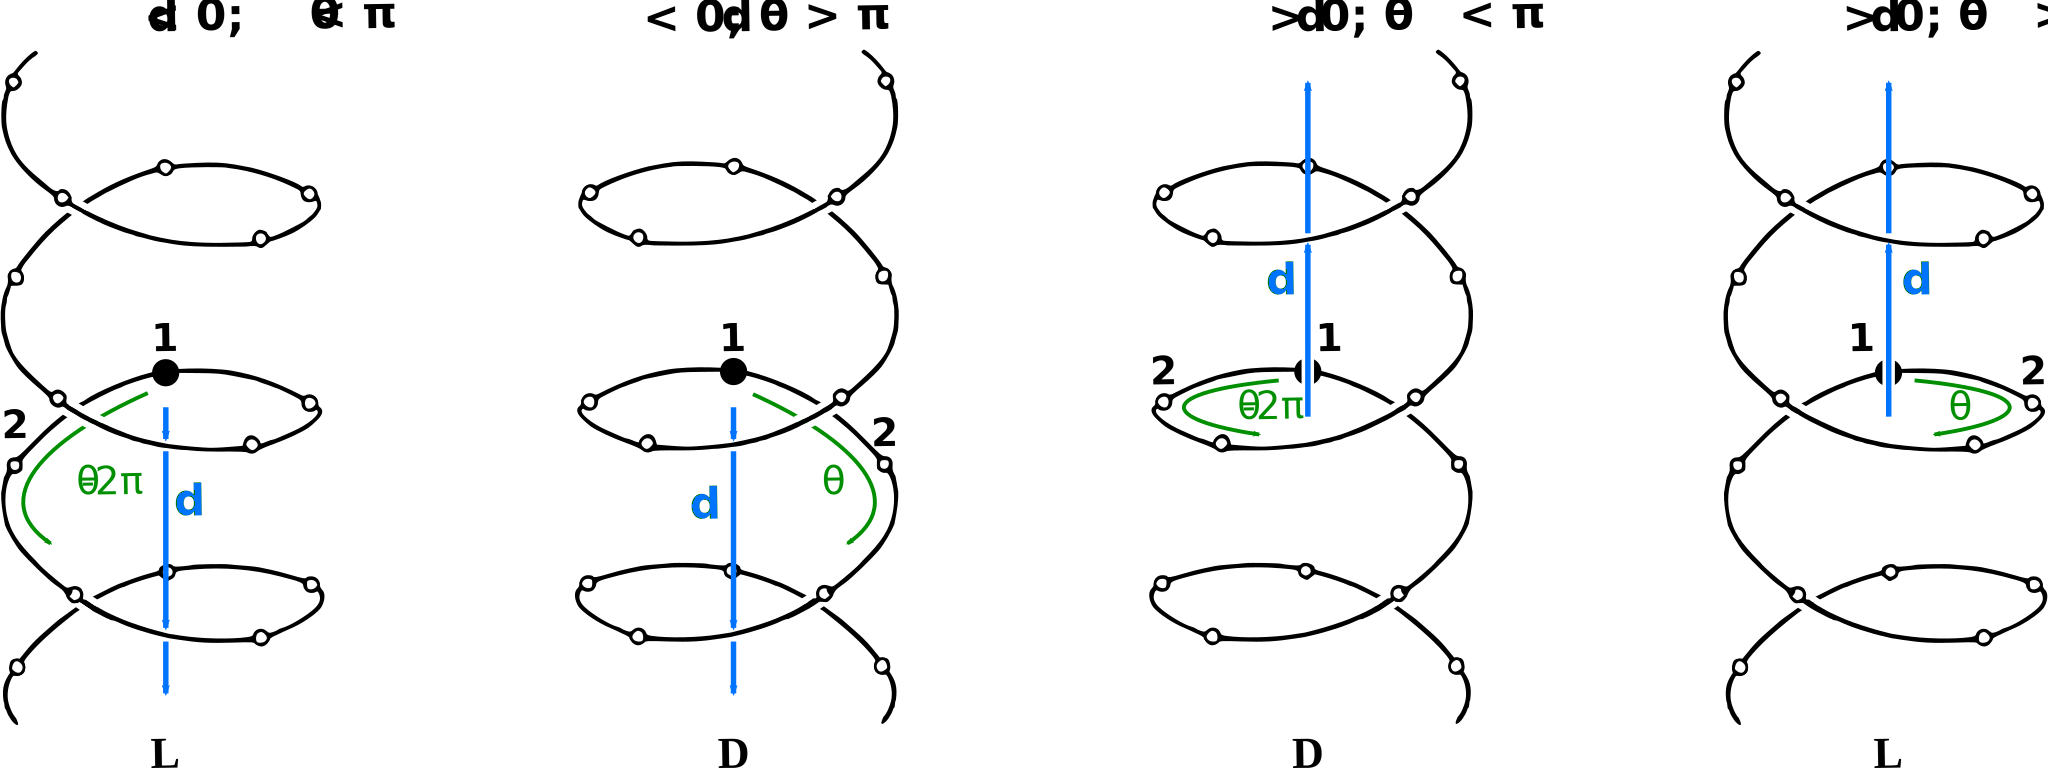
\includegraphics[width=0.95\linewidth]{./figures/helix_handedness.pdf}
\caption{\label{fig:helix_handedness} The handedness of a helix is a function of angular displacement \n{$\theta$} perpendicular to the helical axis (green curved arrows) and linear displacement \n{$d$} along the helical axis (blue, vertical arrows). Note that left-handed \n{(L)} and right-handed \n{(R)}  backbone twists are respectively associated with the L and D chiralities within the Fisher Projection system and S and R chiralities within the Cahn--Ingold--Prelog system \citep{Cross2013}; however, as discussed in the Methods section, this report makes a distinction between helix handedness and molecular chirality.
}
\end{figure}

\n{Given these relationships, this paper proposes a new} metric for backbone handedness that depends on the sign of $d$ and the value of $\theta$:
\begin{equation}\label{eqn:chi}
\h = \frac{d}{\lvert d \rvert} \sin(\theta).
\end{equation}
\n{The range of $\h$ is $[-1,1]$, with negative (or positive) values indicating that the overall twist of the backbone is left(or right)-handed. Also, $|h|$ is proportional to the extent to which the backbone is twisted.} Note that $d/\lvert d \rvert$ is {\em related} to the traditional sign function $\textrm{sgn}(d)$, but deviates at $d=0$, where the former term is undefined while the latter term is 0. Additionally, $\h$ will equal 0 if $d=0$ or if $\theta=x\uppi$ (where $x$ is an integer); for more on the meaning of $d$ and $\theta$ in context of handedness and peptide geometry, please refer to the Results and Discussions section and \Fig{fig:d_vs_theta} in particular. 

\subsection*{Alternative measures of handedness} 

Two estimates for chirality, $\chi_1$ and $\chi_2$, used to validate the new measure of handedness $\h$ (\Eqn{eqn:chi}), were previously used by \cite{Kwiecinska2005} and \cite{Kabsch1983}, respectively. The equations are: 
\begin{equation} \label{eqn:chi1}
\chi_1 = \frac{1}{N}\sum_{i = 2}^{N-2} \frac{(\textit{\textbf{v}}_{i-1} \times \textit{\textbf{v}}_{i})\cdot \textit{\textbf{v}}_{i+1}}{\textit{v}_{i-1} \textit{v}_{i} \textit{v}_{i+1}},
\end{equation}
\begin{equation}\label{eqn:chi2}
\displaystyle \chi_2 = \frac{1}{N}\sum_{i = 2}^{N-2}
 \textrm{arctan2}\left (\textit{v}_i \textit{\textbf{v}}_{i-1} \cdot \textit{\textbf{v}}_i \times \textit{\textbf{v}}_{i+1},\textit{\textbf{v}}_{i-1}\times \textit{\textbf{v}}_i \cdot \textit{\textbf{v}}_i\times \textit{\textbf{v}}_{i+1} \right ).
\end{equation}

Here, $N$ is the peptide length, $i$ is the peptide residue number and the position of each $\upalpha$-carbon is $\textit{\textbf{N}}_i$, with vector $\textit{\textbf{v}}_{k} \equiv \textit{\textbf{N}}_{k+1} - \textit{\textbf{N}}_{k}$. 
%Vector $\textit{\textbf{v}}_{ij} \equiv \textit{\textbf{N}}_{i} - \textit{\textbf{N}}_{j}$ and $\textit{\textbf{v}}_{k} \equiv \textit{\textbf{v}}_{k+1,k} = \textit{\textbf{N}}_{k+1} - \textit{\textbf{N}}_{k}$. 
The scalar component of the vector $\textit{\textbf{v}}_i$ is denoted as $\textit{v}_i$. 
\Eqn{eqn:chi1} has range $[-1,1]$. \Eqn{eqn:chi2}, also used by \cite{Gruziel2013}, is the dihedral angle associated with the four contiguous $\upalpha$-carbons (one preceding and two succeeding the residue $i$), and ranges between $[-\uppi,\uppi]$ radians. For both metrics, values  deviating more from 0 are more chiral (or `twisted' or `handed'), and left-handed twists are negative while right-handed twists are positive. Only $
\upalpha$-carbon atom positions are used for the calculation. 

Finally, a more backbone-agnostic metric of chirality has been introduced by \cite{Solymosi2002}, which is replicated here purely for completeness:
\begin{equation}\label{eqn:chi3}
\displaystyle \chi_3 = \frac{4!}{3N^4} \sum_{i,j,k,l \in \textit{\textbf{N}}} \frac{\left((\textit{\textbf{v}}_{ij} \times \textit{\textbf{v}}_{kl}) \cdot \textit{\textbf{v}}_{il}\right) (\textit{\textbf{v}}_{ij} \cdot \textit{\textbf{v}}_{jk}) (\textit{\textbf{v}}_{jk} \cdot \textit{\textbf{v}}_{kl})} {\left(\textit{v}_{ij} \textit{v}_{jk} \textit{v}_{kl}\right)^2 \textit{v}_{il}}.
\end{equation}
$\chi_3$, of arbitrary range, is known as the chirality index $G_{0S}$ in \cite{Solymosi2002} and \cite{Neal2003}. $(i,j,k,l)$ are exhaustive permutations of $\{1,2,\ldots,N\}$. This metric qualitatively matches the values of \Eqns{eqn:chi1} and~\ref{eqn:chi2}, and, while not shown, the relationship between $(\phi,\psi)$ and $\chi_3$ is available in the online GitHub repository.

\subsection*{Backbone structure generation}
The metric $\h$ (\Eqn{eqn:chi}) is purely analytical and does not need structures to be computationally generated, since \Eqns{eqn:theta_trans} through~\ref{eqn:d_cis} that provide $d$ and $\theta$ require only pairs of $\phi$ and $\psi$ angles. However, if values for bond angles, lengths and dihedral angles are expected to deviate greatly from equilibrium values, $\theta$ and $d$ can only be obtained from the more detailed \Eqns{eqn:theta} and~\ref{eqn:d}, whose parameters would likely be obtained from a structure. On the other hand, as $\chi_1$ (\Eqn{eqn:chi1}) and $\chi_2$ (\Eqn{eqn:chi2}) work explicitly with atom positions, these metrics explicitly need the generation of structures. In order to use these metrics, peptides (poly-glycines) of arbitrary length were generated using the Python-based PeptideBuilder library \citep{Tien2013}. 
Analysis was performed using BioPython \citep{Cock2009} and Numerical Python \citep{VanDerWalt2011}. Ramachandran plots that describe chirality (e.g., \Fig{fig:chi}a) were generated using a grid spacing (in degrees) of $\phi,\psi \in \{-180,-178,\ldots,178,180\}$.

\subsection*{Obtaining secondary structure statistics}
Statistics about secondary structures -- particularly $\alpha$-helices, $3_{10}$-helices and $\beta$-sheets -- %used in \n{\Fig{fig:intro}b and \Fig{fig:alternatives}} 
were identified using the DSSP algorithm \citep{Kabsch1983}, although the STRIDE algorithm \citep{Frishman1995} provides qualitatively identical distributions. \n{The DSSP} algorithm was applied to a database of 13,760 three-dimensional protein conformations (one domain per conformation) with lower than 40\% sequence identity, obtained from the Structural Classification of Proteins or SCOPe website [Release 2.06; \cite{Fox2014}]. This database is currently available as: \url{http://scop.berkeley.edu/downloads/pdbstyle/pdbstyle-sel-gs-bib-40-2.06.tgz}.

\begin{figure}[t!]
%\begin{adjustwidth}{-1in}{0in} % Comment out/remove adjustwidth environment if table fits in text column.
\centering
\includegraphics[width=1.0\linewidth]{./figures/dtheta_full3.pdf}
\caption{\label{fig:d_vs_theta} Further discussion on the meaning of $d$ and $\theta$. As shown in \Fig{fig:helix_handedness}, axial separation $d$ and angular separation $\theta$ between adjacent atoms of the same type combine to define handedness. The \n{brown (dark) and gold (light)} shaded \n{quadrants} within the graph show the distribution of handedness as a function of $d$ and $\theta$. The relevant boundaries -- $\theta=x\uppi$ (where $x$ is a non-negative integer) and $d=0$ -- separate the map into four quadrants of left- and right-twisting backbones (`L' and `R', respectively).  Geometric interpretations of various boundaries, discussed in the text, are shown to the top and left of the graph \n{as three scenarios}. The toroid enclosed by two solid lines (and shaded white) represents all possible conformations for \trans peptides ($\omega=180 \pm 5^\circ$). Similarly, the region allowed for \cis peptides ($\omega=0 \pm 5^\circ$) are bound by the two dashed contours. %As expected, \trans and \cis peptides behave very differently, further predicating the need to explore the two types of backbones as distinct.
}
%\end{adjustwidth}
\end{figure}

\subsection*{Backbone chirality $\bm\neq$ backbone handedness}
Finally, it is important to recognize the distinction between backbone (twist) handedness and backbone (molecular) chirality. Na{\"i}vely, chirality is a simple concept: a molecular conformation is achiral if its mirror image can be superimposed onto itself, otherwise that conformation is chiral \citep{Gold1997} (alternatively, and less commonly, achiral molecules possess inversion centers). Despite this intuitive definition, chirality has remained a confusing concept ever since its introduction \citep{Bentley2010,Wallentin2009}, which is possibly due to the fact that `context' is very important when discussing chirality \citep{Mislow2002}. For example, when looking at a peptide at the residue or `local' level, every amino acid (excepting glycine) is chiral due to the presence of a chiral $\alpha$-carbon (its mirror image can not be superimposed onto itself). Yet, at the macromolecular level, even an all-glycine (and therefore locally achiral) peptide will display {\em conformations} that are not superimposable onto each other, and so such conformations would be chiral. Alternatively, when considering handedness, if a backbone is completely flat (say, a ring, where $d=0$), handedness ($h$) will be undefined, and so one can not speak of handedness of the twist. Yet, the backbone may still remain chiral; e.g., cisplatin and transplatin are planar molecules that are nonetheless chiral opposites \citep{Testa2013}. It is for this reason that this report chooses to be careful to not claim that \Eqn{eqn:chi} is a metric for peptide/backbone chirality, but of peptide backbone {\em twist} handedness. However, estimates for backbone chirality (e.g., \Eqns{eqn:chi1} and~\ref{eqn:chi2}) may be used as surrogates for twist chirality to validate $\h$ (\Eqn{eqn:chi}), as both are related but not the same.

\section*{Results and Discussion}

\subsection*{Relevance of $\bm \theta$ and $\bm d$}

When discussing peptide backbones, two possible definitions of backbone `flatness' (or linearity) are possible: flatness at a residue level and flatness at the atomic level. In the former, all atoms of the same {\em type} are coplanar (examples of atom types are the backbone nitrogens, carbonyl carbons, $\upalpha$-carbons, or even sidechain $\upbeta$-carbons). In the latter \n{definition of flatness}, {\em all} atoms within the backbone are coplanar. For the discussions below, \n{since the} residue-by-residue behavior of the peptide is of primary relevance, the former definition is chosen as the relevant scope for flatness. 

As described in \Fig{fig:helix_handedness}\n{,} the helical parameters $d$ and $\theta$ respectively refer to \n{an axial} displacement along the helical axis and an angular displacement in a plane perpendicular to the helical axis. For example, $d=0$ indicates a helix flattened along its helical axis (\Fig{fig:d_vs_theta}\n{, Scenario 1}). This means that all regular peptides with $d=0$ will be ring-like at some peptide length (shown in a following figure for a range of peptides). As expected from \Eqn{eqn:chi}, at $d=0$, one can not tell how the helix was built, since coplanar peptides can not be described as either left- or right-twisting. Therefore, even though $d=0$ indicates highly twisted peptides, these twists do not possess handedness. This shows up in the $\h$ metric because, at $d=0$, \n{$|d|^{-1}$} is undefined.


\begin{figure}[t!]
\begin{adjustwidth}{-1in}{0in} % Comment out/remove adjustwidth environment if table fits in text column.
\centering
\includegraphics[width=0.9\linewidth]{./figures/chi_snapshots.pdf}
\caption{\label{fig:chi} The \n{handedness} of an ordered \trans peptide within the Ramachandran plot. Panel (a) displays the relationship between backbone parameters $(\phi,\psi)$ and the associated helix parameters of curvature $\sin(\theta)$ (top; \Eqn{eqn:theta}) and \n{axial displacement} $d$ (bottom; \Eqn{eqn:d}). As shown in \Fig{fig:helix_handedness}, the handedness of a helix is a function of these two variables ($\h$; \Eqn{eqn:chi}). Panel (b) is a map of backbone chirality ($\h$) as a function of $\phi$ and $\psi$. The boundaries, $\theta = \uppi$ (`\protect\dashedrule') and $d=0$ (`\protect\dotdashedrule'), correspond to backbones that are equally flat, but which are respectively optimally extended and curved (see discussion in text). 
\n{Panel (b)} shows that the na{\"i}ve expectation of handedness in a Ramachandran plot (\Fig{fig:intro}d) is inaccurate.  Interestingly, our na{\"i}ve expectations would be upheld if one were only to have sampled regions of the Ramachandran plot dominated by known proteins (a; regions enclosed by `\protect\dottedrule' indicate 90\% occupancy). An example of the behavior of one `slice' of (b) is shown in (c). Each snapshot represents a peptide backbone that is either in a distinct region of handedness or at a boundary.
}
\end{adjustwidth}
\end{figure}

\begin{figure}[t!]
\begin{adjustwidth}{-1in}{0in} % Comment out/remove adjustwidth environment if table fits in text column.
\centering
\includegraphics[width=0.9\linewidth]{./figures/various_chis.pdf}
\caption{\label{fig:chi_all} 
Panels (a) and (b) describe the handedness of backbone twists whose amide dihedral angles are \trans ($\omega=\uppi$) and \cis ($\omega=0$), respectively. Column \textit{(i)} describes handedness (\n{$\h$;} \Eqn{eqn:chi}), which does not require structures to be computationally generated. Columns \textit{(ii)} and \textit{(iii)} respectively show vector-based estimates of backbone handedness -- $\chi_1$ (\Eqn{eqn:chi1}) and $\chi_2$ (\Eqn{eqn:chi2}) -- which are calculated from computationally generated peptides (see Methods). Regions of left- and right-handedness are identical for all measures \textit{(i--iii)}. \n{A cartoon representation of distinct regions of handedness is shown in \textit{(iv)}.}  Finally, Panel (c) displays a range of regular \cis peptide backbones with $d\approx0$. As explained \n{in} \Fig{fig:d_vs_theta}, $d=0$ indicates \n{a flat backbone that lies perpendicular to the helical axis, which results in ring-like peptides}. Interestingly, a point in the Ramachandran plot exists exclusively for \cis peptides, where $d=0$ and $\theta=\uppi$: $\phi=-\psi=\pm 36^\circ$ [`\FiveStarOpen' in Panels(b)-\textit{(iv)} and (c)]. }
\end{adjustwidth}
\end{figure}

Additionally \Fig{fig:d_vs_theta} describes two important values for $\theta$: $e\uppi$ \n{(Scenario 2)} and $o\uppi$ \n{(Scenario 3)}, where $e$ and $o$ are even and odd integers. In particular, for any $d$, $\theta=e\uppi$ indicates zero angular displacement along the axis, which puts all atoms of the same type on the same line parallel to the helical axis (\Fig{fig:d_vs_theta}\n{, Scenario 2}). Similarly, $\theta=o\uppi$ indicates that every alternate atom (of the same type) along the backbone will be linear, and every adjacent atom will be diametrically opposite to each other (\Fig{fig:d_vs_theta}\n{, Scenario 3}); i.e., $\theta=o\uppi$ indicates that all atoms of the same type will lie on a plane that is parallel to the helical axis. In short, $\theta=0$ codes for backbones that are linear (optimally extended for a fixed $d$) and $\theta=\uppi$ describe peptides that zig-zag along a plane perpendicular to the helical axis (for a fixed $d$). Finally, as \n{is} evident in \Fig{fig:d_vs_theta}, $\theta=e\uppi$ conformations are not available \n{to} peptide backbones\n{. Therefore}, $\theta=o\uppi$ (e.g., $\uppi$ or $180^\circ$) will be the most extended type of backbone (for a fixed $d$). These relationships show how, {\em a priori}, the curve of a backbone with particular $(d,\theta)$ may be interpreted. 

Finally, $\theta$ may serve as an important single-number metric for describing backbone configurations. \cite{Mannige2016} developed one such number -- a Ramachandran number ($\mathcal{R}$) -- that \n{is a structurally meaningful combination of} $\phi$ and $\psi$. This number depends on the fact that structural features of the backbone (e.g., radius of gyration) vary least when one slices through the \trans Ramachandran plot along negative-sloping lines that conserve $\phi+\psi$ \citep{Ho2003,Zacharias2013,Mannige2016}. Interestingly, $\theta$ follows that trend too, which -- in combination with the fact that regions of the Ramachandran plot are sparse \citep{Mannige2016} -- means that $\theta$ and its derivatives (e.g., $\h$) are {\it universal} Ramachandran numbers. The universality arises from the fact that \cis Ramachandran plots do {\it not} conserve structure along lines that conserve $\phi+\psi$ (and so $\mathcal{R}$ only works for \trans backbones), yet any two backbones with nearly identical $\theta$'s will also be conserved in structure (see, e.g., \Fig{fig:chi}a, top). This feature of $\theta$ will be true irrespective of the nature of the amide dihedral angle $\omega$ (\Eqn{eqn:theta}).

\subsection*{Handedness of \textit{trans} backbones}

\Fig{fig:chi}a describes the behavior of $\sin(\theta)$ and $d$ as a function of $\phi$ and $\psi$ (assuming an all-\trans backbone; $\omega=\uppi$ or $180^\circ$). \Fig{fig:chi}b describes the behavior of \n{backbone} handedness ($\h$; \Eqn{eqn:chi}) as a function of $\phi$ and $\psi$. This map is a complete description of the handedness of an all-\trans (regular) peptide backbone. \Fig{fig:chi}c describes some structures at various regions within the plot. As discussed above, $d=0$ (`\FiveStarOpen) indicates that each residue is at the same `altitude', i.e., the helix is perfectly flat and maximally curved (at that particular $\theta$). Note that any path on the Ramachandran plot that transitions from negative to positive $d$ will encounter an infinitesimal region in its path \n{where} $d=0$ \n{and so $\h$ is undefined. This, along with the recognition that $d=0$ indicates highly curved backbones, means that such transitions would be concomitant with a sharp change in handedness}. When $\theta=\uppi$, then the backbone is also flat (see `\FiveStar' in \Fig{fig:chi}c); however, atoms of the same type lie in a single plane that is perpendicular to the helical axis (\Fig{fig:d_vs_theta}). In short, within the Ramachandran plot, $d=0$ (`\protect\dotdashedrule') and $\h=\uppi$ (`\protect\dashedrule') code for {\it flat} backbones that are respectively either optimally curved (at a given $\theta$) or optimally extended (at a given $d$). A future report will discuss how these simple rules may be combined to make conjectures about novel secondary and tertiary structures.

\Fig{fig:chi_all}a shows that the equation for $\h$ match other metrics for handedness, as interpreted by other metrics for chirality \citep{Kwiecinska2005,Kabsch1983,Gruziel2013}. In particular, \Fig{fig:chi_all}a displays the Ramachandran plot colored by $\h$ [\textit{(i)}; \Eqn{eqn:chi}] next to estimates calculated using $\chi_1$ [\textit{(ii)}; \Eqn{eqn:chi1}] and $\chi_2$ [\textit{(iii)}; \Eqn{eqn:chi2}]. Each panel describes identical regions of left- and right-handedness, which is shown as a cartoon in \textit{(iv)}. However, given that $\chi_1$ and $\chi_2$ are estimates of chirality and not backbone handedness, their exact values differ from the primary metric for handedness ($\h$) provided here.

\subsection*{Handedness of \textit{cis} backbones}
In the same vein as \Fig{fig:chi_all}a, \Fig{fig:chi_all}b displays $\h$, $\chi_1$ and $\chi_2$ as a function of $\phi$ and $\psi$ for all-\cis regular backbones. This appears to be the first complete description of chirality of an all-\cis backbone ($\omega=0$). Interestingly, the boundaries for $d=0$ and $\theta=\uppi$ switch in \cis backbones, with the -ve diagonal and curved boundaries being caused by $d$ and $\theta$, respectively. Additionally, \Fig{fig:chi_all}a reiterates the idea that \cis peptides are quite different when compared to \trans peptides: the regions and boundaries of left- and right-handedness within the Ramachandran plot differ for \cis versus \trans. 

Finally, points on the \cis map ($\phi=\pm36^\circ$, $\psi=\mp36^\circ$) exist where $d=0$ {\em and} $\theta=\uppi$. An example of this, along with other $d=0$ configurations, is shown in \Fig{fig:chi_all}c for a six-residue peptide. At first glance, this appears to be contradiction, because $d=0$ indicates the most curved backbone at a fixed $\theta$, and $\theta=\uppi$ indicates the most linear backbone at a fixed $d$\n{; however, it is purely due to the nature of the $cis$ backbone that this indeed is possible.} Of course, this structure would only be possible for cyclic peptides with length two, given that any peptoid of length greater than two would result in overlapping atoms. However, such a structure (one with $d=0$ and $\theta=\uppi$) is not possible in \trans peptides, even in theory, because the boundaries associated with $d=0$ and $\theta=\uppi$ do not intersect (\Fig{fig:chi_all}a); this is also evident in \Fig{fig:d_vs_theta}, where \trans peptides are shown to not occupy regions of $(d,\theta)$ = $(0,\uppi)$, while \cis peptides do.

%\subsection*{How does the amide backbone ($\bm\omega$) change the chirality landscape?}
\n{The exhaustive survey of regular \cis ($\omega=0$) and \trans ($\omega=\uppi$) peptides (\Fig{fig:chi_all}) proves that the na{\"i}ve picture of chirality -- that the -ve diagonal separates the right-twisting backbones from the left-twisting backbones (\Fig{fig:intro}d) -- is wrong.} However, deviations from $\omega = 0$ or $\uppi$ are evident in the Protein Databank; see, e.g., discussions by \cite{Improta2011}. \n{This raises the question:  how does varying $\omega$ through non-traditional values change the handedness landscape?} \Fig{fig:omega_range} describes Ramachandran plots that show \n{handedness} in terms of varying $\omega$\n{, which shows that this complicated separation of handedness in \cis and \trans backbones also holds for other values of $\omega$. Therefore, the} na{\"i}ve expectation of handedness (\Fig{fig:intro}d) is too simple, irrespective of amide dihedral angle.

\begin{figure}[t!]
%\centering
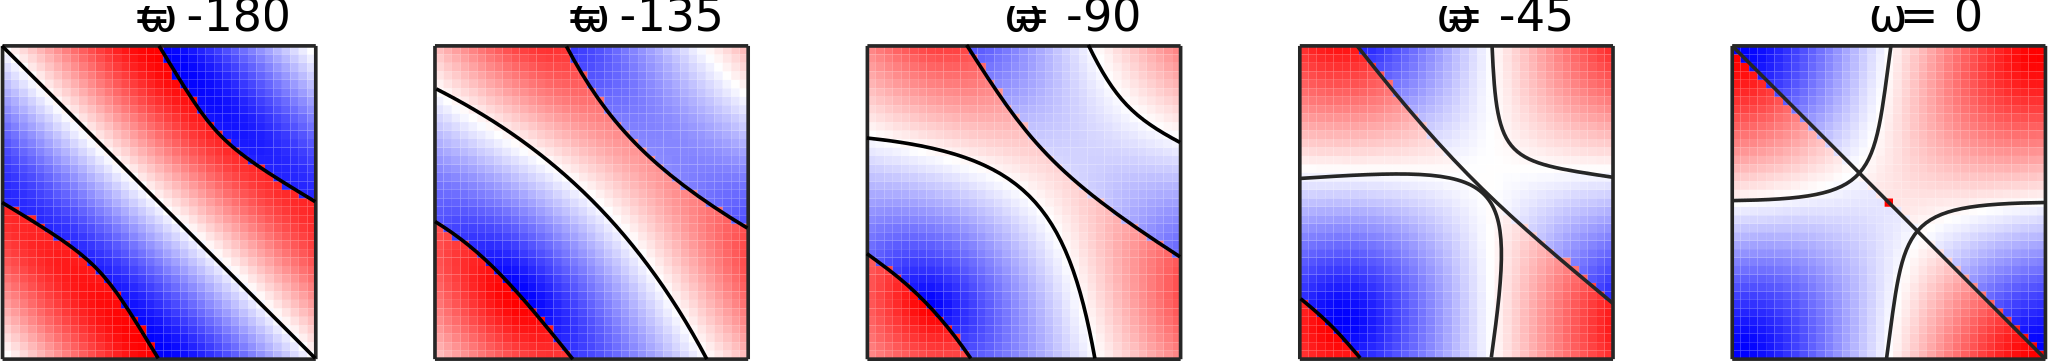
\includegraphics[width=0.95\linewidth]{./figures/various_omegas.pdf}
\caption{The landscape of backbone chirality as a function of amide dihedral angle $\omega$. As $\omega$ is changed, the features of the landscape smoothly transform from the landscapes of $\omega=\pm\uppi$ to $\omega=0$. For all values of $\omega$, it is evident that the na{\"i}ve view of chirality (\Fig{fig:intro}d) is wrong: at least four distinct regions of chirality (separated by boundaries $d=0$ and \n{$\theta=\uppi$}) are evident in each scenario. Although only five snapshots (values of $\omega$) are shown, all integer values of $\omega$ were tested, which 
corroborates the fact that the na{\"i}ve view of backbone handedness (\Fig{fig:intro}d) is universally incorrect.
\label{fig:omega_range}}
\end{figure}

\begin{figure}[b!]
\centering
\includegraphics[width=\linewidth]{./figures/various_chis_skewed.pdf}
\caption{\label{fig:other_chis_skewed} \n{The two frames of reference (or ranges) for the Ramachandran plot for \trans and \cis backbones.} Both ranges $[-\uppi,\uppi\n{)}$ and $[0,2\uppi\n{)}$ yield similar trends for \trans backbones (a,b); however, for \cis backbones, the latter frame of reference (d) appears to more neatly apportion the handedness of the backbone rather than the traditional frame of reference (c). As in \Figs{fig:chi} and~\ref{fig:chi_all}, `\protect\dashedrule' and `\protect\dotdashedrule' respectively correspond to boundaries defined by $\theta = \uppi$ and $d=0$. Also, regions bound by dotted contours indicate dominant regions within which proteins reside ($p=0.9$).}
\end{figure}

\subsection*{[$\bm{-\uppi}$,$\bm{\uppi}$) or [$\bm{0}$,$\bm{2\uppi}$): which frame of reference to use?} 
In structural biology, $\phi$ and $\psi$ within the Ramachandran plot has been historically set to range between the values $[-\uppi,\uppi)$ radians [see, e.g., textbooks by \cite{Berg2006} and \cite{Alberts2002}]. However, \cite{Ramachandran1963} had originally used the range of $[0,2\uppi)$. Today, the range $[-\uppi,\uppi)$ is used predominantly by structural biologists \citep{Laskowski1993,Laskowski2003,Zacharias2013}, while some have turned to $[0,2\uppi)$ as the norm \citep{Nemethy1966,Voelz2011}. 

Given the periodicity of the Ramachandran plot, \n{the two frames of reference are scientifically identical}; however the value of the Ramachandran plot \n{lies in its utility as a {\em map}}: it is a map of important features of proteins relative to the various regions, quadrants, and diagonals in the map [see, e.g., discussions by \cite{Beck2008}]. The Ramachandran plot's value lies in being able to convey large amounts of information in easy to read pictograms. For that reason, switching the map from one range to another means that the two types of scientists \n{-- each used to a distinct range --} will not be able to converse as seamlessly.

Therefore, the following question must arise: which range -- $[-\uppi,\uppi\n{)}$ or $[0,2\uppi\n{)}$ -- is able to convey more information with the least amount of effort? \Fig{fig:other_chis_skewed} shows the \n{handedness} of a \trans backbone (a,b) and \cis backbone (c,d) in the two frames of reference. From (a) and (b) it is evident that general trends in the map for \trans backbones remain the same in both frames of reference: the negative diagonal ($\theta=\uppi$) locally separates right-handed regions from left-handed regions, while the curved line ($d=0$) -- which also separates handedness -- also appears to be in generally the same regions (albeit inverted in curvature). The \cis backbones, however, look dramatically different in the two frames of reference: the range $[-\uppi,\uppi]$ separates handedness in a more complicated manner (c), while, for the most part, the -ve diagonal appears to meaningfully separate handedness when the plot ranges from $0$ to $2\uppi$ (d). For this reason, purely when looking at handedness, and especially in the case of \cis backbones, the Ramachandran plot that ranges between 0 and $2\uppi$ appears to be more meaningful.
%\cite{Laskowski1993,Laskowski2003,Zacharias2013,Mannige2016}
%The Ramachandran plot has been displayed to students of structural biology primarily in the range of $[-\uppi,\uppi]$\cite{Berg2006,Alberts2002}. 
%range between $-\uppi$ and $\uppi$\footnote{An angle $\zeta$ can be wrapped within the range $[-180,180)$ using $\zeta' = - 180 + (\zeta + 180) \% (360)$, where $\%$ represents the modulus function.}

\begin{figure}[t!]
\begin{adjustwidth}{-1in}{0in} % Comment out/remove adjustwidth environment if table fits in text column.
\centering
\includegraphics[width=1.0\linewidth]{./figures/various_2d_distributions.pdf}
\caption{\label{fig:alternatives} 
Alternative representations of the Ramachandran plot. While the Ramachandran plot is useful to map characteristics of secondary structures (a), it is not intuitive. For example, the relationship between the Ramachandran parameters $(\phi,\psi)$ and the handedness of a backbone is not obvious (see, e.g., the non-obvious distribution of left- and right-handed peptides as a function of $\phi$ and $\psi$). For this reason, \cite{Zacharias2013} introduced a graphical format involving the helical parameters $d$ and $\theta$ in polar coordinate space (b), where the regions of left- and right-handedness are obvious [their format differs from (b) in that their $\theta$ increases in counter-clockwise fashion]. Panel (c), which is an extension of \Fig{fig:d_vs_theta}, introduces another graphical representation of backbone degrees of freedom based on $(\theta,d)$, but  in Cartesian space. While both (b) and (c) are equally useful in understanding regions available to a protein, the text discusses some benefits of (c) as a universal map for exploring new conformations and secondary structures. Excepting the left-handed helices ($\upalpha_\textrm{L}$-, $3_\textrm{10L}$-helices\n{; see Methods}), each secondary structure has two contours signifying $p=0.5$ and $0.8$.
}
\end{adjustwidth}
\end{figure}

\subsection*{A universal alternative to the Ramachandran plot}
While the Ramachandran plot is useful enough to earn a place in undergraduate-level biology textbooks \n{\citep{Berg2006,Alberts2002}}, as discussed throughout this report, it is not easy to estimate features of a peptide backbone just from its $(\phi,\psi)$ angles (\Fig{fig:alternatives}a). This prompted \cite{Zacharias2013} to introduce a new representation for backbone degrees of freedom in the form of a polar graph. In this polar representation, the $\theta$ is the angular coordinate (azimuth) and $d$ is the radial coordinate. An example of one such representation is shown in \Fig{fig:alternatives}b, with the direction of increasing $\theta$ reversed (compared to the cited report) to maintain relative positions of secondary structures within the Ramachandran plot (\Fig{fig:alternatives}a). \cite{Zacharias2013} stated an additional reason for the introduction of the polar representation (\Fig{fig:alternatives}b): $\theta$, which is an angle and therefore periodic, can remain periodic as the angular coordinate in the graph. 

However, the format proposed by \cite{Zacharias2013} (\Fig{fig:alternatives}b) is incomplete for a few reasons: 1) $d<0$ peptides (the bottom-left and top-right regions of \Fig{fig:chi}a, bottom) will never be observed in this map since only structures with $d \geq 0$ are allowed; 2) all peptides with $d=0$ (marked by `\dotdashedrule' in every preceding Ramachandran plot) will be compressed into one point at the center, even though \Fig{fig:chi_all}c shows a range of legitimate $d=0$ conformations; 3) while the graph is $\theta$-periodic, the values for $\theta$ in peptides are constrained within one $[0,2\uppi]$ period (peptides range between $\theta=\uppi/4$ and $2\uppi - \uppi/4$; vertical dotted lines in \Fig{fig:d_vs_theta}); i.e., periodicity in $\theta$ is not required for the faithful representation of peptides. Fortunately, even though this system is not universal (again, since $d<0$ structures are not accommodated), most conformations in globular proteins display positive $d$, and so the representation presented by \cite{Zacharias2013} is a reasonable one for most proteins with known structure.

Interestingly, \Fig{fig:alternatives}c -- which arranges the parameters $\theta$ and $d$ along Cartesian axes -- serves as both a universal {\em and} intuitive map for peptide backbone geometry. This is because: 1) as shown in \Fig{fig:d_vs_theta}, such maps reveal a wealth of information about the peptide backbone, 2) both positive and negative values of $d$ are allowed (compared to \Fig{fig:alternatives}b), due to the shift in the coordinate system from polar to Cartesian, and 3) this format accommodates {\it every} type of peptide conformation: any peptide (or its mimic) has a place in this map irrespective of whether the amide backbone is \cis or \trans or any other value; additionally, if the backbone is distorted, such distortions can also be accounted for since $d$ and $\theta$ \n{account for} such distortions (\Eqns{eqn:theta} and~\ref{eqn:d}). This is impossible to do using a single Ramachandran plot without making sweeping assumptions about backbone parameters that are not $\phi$ and $\psi$. The $(\theta,d)$ plot opens up the possibility for a new, intuitive, and {\it universal} kind of graphical representation as a supplement to the Ramachandran plot.

\subsection*{A departure from perfect regularity}
So far, this report has focused on regular or {\em simple}  backbone conformations, i.e., those that are formed from the same $\phi$ and $\psi$ angles repeated along the backbone. This is particularly because a simple and visually intuitive correspondence exists (\Figs{fig:helix_handedness} and~\ref{fig:d_vs_theta}) between a regular backbone (described by myriad internal coordinates) and a helix that is described simply by $(d,\theta)$. 
%This simple correspondence allows for an intuitive understanding as to how to envision regular backbones as a function of $d$ and $\theta$ (\Figs{fig:helix_handedness} and~\ref{fig:d_vs_theta}). 
However, there is a possibility that $d$ and $\theta$ are useful even in isolation, when the unreasonable constraint of perfect backbone regularity is lifted. An example of such a departure from regularity follows. 

Some secondary structures are characterized by the regular combination of two or more sets of $[\phi,\psi]$ \citep{Pauling1951a, Pauling1951b, Armen2004, Daggett2006, Hayward2008, Mannige2015, Mannige2016}. For example, the $\Sigma$-strand is constructed by alternating between two backbone states $(\phi,\psi,\omega)=(-A,B,180^\circ)$ and $(-B,A,180^\circ)$, where $A \approx 120$ and $B \approx 90$ [Fig.~4h in \cite{Mannige2015}]. It was found that the two states are similar in the extent to which the backbone twists, but opposite in handedness, which allows for these secondary structures to remain linear, albeit in a meandering way \citep{Mannige2015}. \Eqn{eqn:chi} also describes these two states as opposite in handedness and similar in twist extent: the $\h$ for the two states are $-0.34$ and $0.51$, respectively (the difference in magnitude is within the range of the standard deviation in $\h$ [$0.391$] for the $\upbeta$-sheet). Similarly, the $\upalpha$-sheet proposed by \cite{Pauling1951b} is constructed by alternating between $\upalpha_\textrm{(D)}$ and $\upalpha_\textrm{L}$ backbone states,  yet this motif is linear because each state describes equal but opposite handedness $\h=\pm 0.41$. These points raise the possibility that, even in the absence of perfect backbone regularity, the values $d$\n{,} $\theta$, and \n{$\h$} may be considered to be residue-specific properties that may be combined to readily provide insights about higher order structures. %A future text will focus on the theory behind meaningfully combining non-equal $(d,\theta)$'s in context of irregular structures.

\section*{Conclusions}

This report introduces a metric for backbone handedness ($\h$) that is based on modeling the backbone as a helix [\Fig{fig:helix}; \cite{Miyazawa1961}]. In particular, $\h$, which is a combination of the helical parameters $\theta$ (angular displacement) and $d$ (\n{axial} displacement), ranges from -1 and 1, and is negative (or positive) when the backbone twist is left(or right)-handed (with larger $|\h|$ indicating greater extent of twistedness). This metric ($\h$) was used to characterize every regular backbone's twist \n{within the Ramachandran plot}, for both \cis and \trans peptides. In doing so, this report dispels a na{\"i}ve view of handedness (\Fig{fig:intro}d), which states that backbone handedness in the Ramachandran plot is separated by the negative-sloped (-ve) diagonal. Interestingly, the reason for the na{\"i}ve view makes senses when considering only \trans peptides: the -ve diagonal (`\protect\dashedrule' in \Figs{fig:chi}a) separates $D$ and $L$ twists {\em if} one considers only the regions dominantly occupied by structured proteins (`\protect\dottedrule' in \Figs{fig:chi}a). Plotting the backbone handedness $(\h)$ in the \n{two} common frames of reference -- $\phi,\psi \in [-\uppi,\uppi)$ and $[0,2\uppi)$ -- indicates that the less commonly used frame $[0,2\uppi)$ may be more appropriate for interpreting \cis backbones (\Fig{fig:other_chis_skewed}).

The behavior of a backbone in \cis and \trans Ramachandran plots look dramatically different (\Fig{fig:chi_all}), and so scientists dealing with new structures \n{that have} a combination of \cis and \trans backbones can not use one Ramachandran plot to faithfully describe these structures. Interestingly, the parameters $\theta$ and $d$ combine all features (internal coordinates) of a contorting backbone, including the amide dihedral angle $\omega$, which means that $(\theta,d)$ can describe {\em any} peptide backbone, irrespective of $\omega$. Therefore, the Cartesian plot with $\theta$ and $d$ as the x- and y-axis, respectively, serves as a unique plot for {\em any} peptide backbone (\Fig{fig:alternatives}), with specific values and boundaries containing deep structural meaning (\Fig{fig:d_vs_theta}). These discussions, the author hopes, clarify a number of concepts associated with the Ramachandran plot, while providing new insights into how to interrogate the features of new protein and protein-like structures.

\section*{Acknowledgments}

\n{The author thanks Alana Canfield Mannige, Ronald D. Hills Jr, the editor, and the reviewer for their constructive input.}

%\bibliography{all}
\begin{thebibliography}{60}
\providecommand{\natexlab}[1]{#1}
\expandafter\ifx\csname urlstyle\endcsname\relax
  \providecommand{\doi}[1]{doi:\discretionary{}{}{}#1}\else
  \providecommand{\doi}{doi:\discretionary{}{}{}\begingroup
  \urlstyle{rm}\Url}\fi

\bibitem[{Alberts \emph{et~al.}(2002)Alberts, Johnson, Lewis, Raff, Roberts,
  and Walter}]{Alberts2002}
\textbf{Alberts B, Johnson A, Lewis J, Raff M, Roberts K, Walter P}.
  \textbf{2002}.
\newblock Molecular biology of the cell. new york: Garland science; 2002.
\newblock \emph{Classic textbook now in its 5th Edition} .

\bibitem[{Armen \emph{et~al.}(2004)Armen, DeMarco, Alonso, and
  Daggett}]{Armen2004}
\textbf{Armen RS, DeMarco ML, Alonso DO, Daggett V}. \textbf{2004}.
\newblock Pauling and corey's $\alpha$-pleated sheet structure may define the
  prefibrillar amyloidogenic intermediate in amyloid disease.
\newblock \emph{Proceedings of the National Academy of Sciences of the United
  States of America} \textbf{101(32)}:11622--11627.

\bibitem[{Beck \emph{et~al.}(2008)Beck, Alonso, Inoyama, and
  Daggett}]{Beck2008}
\textbf{Beck DA, Alonso DO, Inoyama D, Daggett V}. \textbf{2008}.
\newblock The intrinsic conformational propensities of the 20 naturally
  occurring amino acids and reflection of these propensities in proteins.
\newblock \emph{Proceedings of the National Academy of Sciences}
  \textbf{105(34)}:12259--12264.

\bibitem[{Bentley(2010)}]{Bentley2010}
\textbf{Bentley R}. \textbf{2010}.
\newblock Chiral: a confusing etymology.
\newblock \emph{Chirality} \textbf{22(1)}:1--2.

\bibitem[{Berg \emph{et~al.}(2010)Berg, Tymoczko, and Stryer}]{Berg2006}
\textbf{Berg JM, Tymoczko JL, Stryer L}. \textbf{2010}.
\newblock \emph{Biochemistry, International Edition}.
\newblock WH Freeman \& Co., New York, 7 edition.

\bibitem[{Berman \emph{et~al.}(2000)Berman, Westbrook, Feng, Gilliland, Bhat,
  Weissig, Shindyalov, and Bourne}]{Berman2000}
\textbf{Berman HM, Westbrook J, Feng Z, Gilliland G, Bhat T, Weissig H,
  Shindyalov IN, Bourne PE}. \textbf{2000}.
\newblock The protein data bank.
\newblock \emph{Nucleic Acids Research} \textbf{28(1)}:235--242.

\bibitem[{Bragg \emph{et~al.}(1950)Bragg, Kendrew, and Perutz}]{Bragg1950}
\textbf{Bragg L, Kendrew JC, Perutz MF}. \textbf{1950}.
\newblock Polypeptide chain configurations in crystalline proteins.
\newblock \emph{Proceedings of the Royal Society of London Series A
  Mathematical and Physical Sciences} \textbf{203(1074)}:321--357.

\bibitem[{Chothia \emph{et~al.}(1997)Chothia, Hubbard, Brenner, Barns, and
  Murzin}]{Chothia1997}
\textbf{Chothia C, Hubbard T, Brenner S, Barns H, Murzin A}. \textbf{1997}.
\newblock Protein folds in the all-beta and all-alpha classes.
\newblock \emph{Annual Review of Biophysics and Biomolecular Structure} \textbf{26}:597--627.

\bibitem[{Cock \emph{et~al.}(2009)Cock, Antao, Chang, Chapman, Cox, Dalke,
  Friedberg, Hamelryck, Kauff, Wilczynski, and de~Hoon}]{Cock2009}
\textbf{Cock P, Antao T, Chang J, Chapman B, Cox C, Dalke A, Friedberg I,
  Hamelryck T, Kauff F, Wilczynski B, de~Hoon M}. \textbf{2009}.
\newblock Biopython: freely available python tools for computational molecular
  biology and bioinformatics.
\newblock \emph{Bioinformatics} \textbf{25(11)}:1422--1423.

\bibitem[{Cooper and Hausman(2013)}]{Cooper2000}
\textbf{Cooper GM, Hausman RE}. \textbf{2013}.
\newblock \emph{The Cell: A Molecular Approach}.
\newblock Sinauer Associates, Inc., Sunderland, MA, 6 edition.

\bibitem[{Cross and Klyne(2013)}]{Cross2013}
\textbf{Cross L, Klyne W}. \textbf{2013}.
\newblock \emph{Rules for the Nomenclature of Organic Chemistry: Section E:
  Stereochemistry (Recommendations 1974)}.
\newblock Elsevier.

\bibitem[{Daggett(2006)}]{Daggett2006}
\textbf{Daggett V}. \textbf{2006}.
\newblock $\alpha$-sheet: the toxic conformer in amyloid diseases?
\newblock \emph{Accounts of Chemical Research} \textbf{39(9)}:594--602.

\bibitem[{Eisenberg(2003)}]{Eisenberg2003}
\textbf{Eisenberg D}. \textbf{2003}.
\newblock The discovery of the $\alpha$-helix and $\beta$-sheet, the principal
  structural features of proteins.
\newblock \emph{Proceedings of the National Academy of Sciences}
  \textbf{100(20)}:11207--11210.

\bibitem[{Engh and Huber(1991)}]{Engh1991}
\textbf{Engh RA, Huber R}. \textbf{1991}.
\newblock Accurate bond and angle parameters for x-ray protein structure
  refinement.
\newblock \emph{Acta Crystallographica Section A: Foundations of
  Crystallography} \textbf{47(4)}:392--400.

\bibitem[{Engh and Huber(2006)}]{Engh2006}
\textbf{Engh R, Huber R}. \textbf{2006}.
\newblock Structure quality and target parameters.
\newblock In \emph{International Tables for Crystallography Volume F:
  Crystallography of biological macromolecules}, pages 382--392. Springer.

\bibitem[{Esposito \emph{et~al.}(2013)Esposito, Balasco, De~Simone, Berisio,
  and Vitagliano}]{Esposito2013}
\textbf{Esposito L, Balasco N, De~Simone A, Berisio R, Vitagliano L}.
  \textbf{2013}.
\newblock Interplay between peptide bond geometrical parameters in nonglobular
  structural contexts.
\newblock \emph{BioMed Research International} \textbf{2013}.

\bibitem[{Ferrarini and Nordio(1998)}]{Ferrarini1998}
\textbf{Ferrarini A, Nordio PL}. \textbf{1998}.
\newblock On the assessment of molecular chirality.
\newblock \emph{Journal of the Chemical Society, Perkin Transactions 2}
  \textbf{(2)}:455--460.

\bibitem[{Fox \emph{et~al.}(2014)Fox, Brenner, and Chandonia}]{Fox2014}
\textbf{Fox NK, Brenner SE, Chandonia JM}. \textbf{2014}.
\newblock Scope: Structural classification of proteins--extended, integrating
  scop and astral data and classification of new structures.
\newblock \emph{Nucleic Acids Research} \textbf{42(Database issue)}:D304--D309.

\bibitem[{Frishman and Argos(1995)}]{Frishman1995}
\textbf{Frishman D, Argos P}. \textbf{1995}.
\newblock Knowledge-based protein secondary structure assignment.
\newblock \emph{Proteins: Structure, Function, and Bioinformatics}
  \textbf{23(4)}:566--579.

\bibitem[{Gold \emph{et~al.}(1997)Gold, Loening, McNaught, and
  Shemi}]{Gold1997}
\textbf{Gold V, Loening K, McNaught A, Shemi P}. \textbf{1997}.
\newblock IUPAC compendium of chemical terminology.
\newblock \emph{Blackwell Science, Oxford} .

\bibitem[{Gorske \emph{et~al.}(2016)Gorske, Mumford, and Conry}]{Gorske2016}
\textbf{Gorske BC, Mumford EM, Conry RR}. \textbf{2016}.
\newblock Tandem incorporation of enantiomeric residues engenders discrete
  peptoid structures.
\newblock \emph{Organic Letters} .

\bibitem[{Gruziel \emph{et~al.}(2013)Gruziel, Dzwolak, and
  Szymczak}]{Gruziel2013}
\textbf{Gruziel M, Dzwolak W, Szymczak P}. \textbf{2013}.
\newblock Chirality inversions in self-assembly of fibrillar superstructures: a
  computational study.
\newblock \emph{Soft Matter} \textbf{9(33)}:8005--8013.

\bibitem[{Harris \emph{et~al.}(1999)Harris, Kamien, and Lubensky}]{Harris1999}
\textbf{Harris AB, Kamien RD, Lubensky TC}. \textbf{1999}.
\newblock Molecular chirality and chiral parameters.
\newblock \emph{Reviews of Modern Physics} \textbf{71(5)}:1745.

\bibitem[{Hayward and Milner-White(2008)}]{Hayward2008}
\textbf{Hayward S, Milner-White EJ}. \textbf{2008}.
\newblock The geometry of $\alpha$-sheet: Implications for its possible
  function as amyloid precursor in proteins.
\newblock \emph{Proteins: Structure, Function, and Bioinformatics}
  \textbf{71(1)}:415--425.

\bibitem[{Ho \emph{et~al.}(2003)Ho, Thomas, and Brasseur}]{Ho2003}
\textbf{Ho BK, Thomas A, Brasseur R}. \textbf{2003}.
\newblock Revisiting the ramachandran plot: Hard-sphere repulsion,
  electrostatics, and h-bonding in the $\alpha$-helix.
\newblock \emph{Protein Science} \textbf{12(11)}:2508--2522.

\bibitem[{Hooft \emph{et~al.}(1997)Hooft, Sander, and Vriend}]{Hooft1997}
\textbf{Hooft RW, Sander C, Vriend G}. \textbf{1997}.
\newblock Objectively judging the quality of a protein structure from a
  ramachandran plot.
\newblock \emph{Computer Applications in the Biosciences: CABIOS}
  \textbf{13(4)}:425--430.

\bibitem[{Iakoucheva \emph{et~al.}(2002)Iakoucheva, Brown, Lawson,
  Obradovi{\'c}, and Dunker}]{Iakoucheva2002}
\textbf{Iakoucheva LM, Brown CJ, Lawson JD, Obradovi{\'c} Z, Dunker AK}.
  \textbf{2002}.
\newblock Intrinsic disorder in cell-signaling and cancer-associated proteins.
\newblock \emph{Journal of Molecular Biology} \textbf{323(3)}:573--584.

\bibitem[{Improta \emph{et~al.}(2011)Improta, Vitagliano, and
  Esposito}]{Improta2011}
\textbf{Improta R, Vitagliano L, Esposito L}. \textbf{2011}.
\newblock Peptide bond distortions from planarity: new insights from quantum
  mechanical calculations and peptide/protein crystal structures.
\newblock \emph{PLoS One} \textbf{6(9)}:e24533.

\bibitem[{Improta \emph{et~al.}(2015{\natexlab{a}})Improta, Vitagliano, and
  Esposito}]{Improta2015}
\textbf{Improta R, Vitagliano L, Esposito L}. \textbf{2015}{\natexlab{a}}.
\newblock Bond distances in polypeptide backbones depend on the local
  conformation.
\newblock \emph{Acta Crystallographica Section D: Biological Crystallography}
  \textbf{71(6)}:1272--1283.

\bibitem[{Improta \emph{et~al.}(2015{\natexlab{b}})Improta, Vitagliano, and
  Esposito}]{Improta2015a}
\textbf{Improta R, Vitagliano L, Esposito L}. \textbf{2015}{\natexlab{b}}.
\newblock The determinants of bond angle variability in protein/peptide
  backbones: A comprehensive statistical/quantum mechanics analysis.
\newblock \emph{Proteins: Structure, Function, and Bioinformatics}
  \textbf{83(11)}:1973--1986.

\bibitem[{Kabsch and Sander(1983)}]{Kabsch1983}
\textbf{Kabsch W, Sander C}. \textbf{1983}.
\newblock Dictionary of protein secondary structure: pattern recognition of
  hydrogen-bonded and geometrical features.
\newblock \emph{Biopolymers} \textbf{22(12)}:2577--2637.

\bibitem[{Kwieci{\'n}ska and Cieplak(2005)}]{Kwiecinska2005}
\textbf{Kwieci{\'n}ska JI, Cieplak M}. \textbf{2005}.
\newblock Chirality and protein folding.
\newblock \emph{Journal of Physics: Condensed Matter} \textbf{17(18)}:S1565.

\bibitem[{Laskowski(2003)}]{Laskowski2003}
\textbf{Laskowski RA}. \textbf{2003}.
\newblock Structural quality assurance.
\newblock \emph{Structural Bioinformatics, Volume 44} pages 273--303.

\bibitem[{Laskowski \emph{et~al.}(1993)Laskowski, MacArthur, Moss, and
  Thornton}]{Laskowski1993}
\textbf{Laskowski RA, MacArthur MW, Moss DS, Thornton JM}. \textbf{1993}.
\newblock Procheck: a program to check the stereochemical quality of protein
  structures.
\newblock \emph{Journal of Applied Crystallography} \textbf{26(2)}:283--291.

\bibitem[{Linderstr{\o}m-Lang(1952)}]{Linderstrom-Lang1952}
\textbf{Linderstr{\o}m-Lang KU}. \textbf{1952}.
\newblock \emph{Lane Medical Lectures: proteins and enzymes}, volume~6.
\newblock Stanford University Press.

\bibitem[{Mannige(2014)}]{Mannige2014b}
\textbf{Mannige RV}. \textbf{2014}.
\newblock Dynamic new world: Refining our view of protein structure, function
  and evolution.
\newblock \emph{Proteomes} \textbf{2(1)}:128--153.

\bibitem[{Mannige \emph{et~al.}(2015)Mannige, Haxton, Proulx, Robertson,
  Battigelli, Butterfoss, Zuckermann, and Whitelam}]{Mannige2015}
\textbf{Mannige RV, Haxton TK, Proulx C, Robertson EJ, Battigelli A, Butterfoss
  GL, Zuckermann RN, Whitelam S}. \textbf{2015}.
\newblock Peptoid nanosheets exhibit a new secondary structure motif.
\newblock \emph{Nature} \textbf{526}:415--420.

\bibitem[{Mannige \emph{et~al.}(2016)Mannige, Kundu, and
  Whitelam}]{Mannige2016}
\textbf{Mannige RV, Kundu J, Whitelam S}. \textbf{2016}.
\newblock The {R}amachandran number: an order parameter for protein geometry.
\newblock \emph{PLoS One} \textbf{11(8)}:e0160023.

\bibitem[{Mirijanian \emph{et~al.}(2014)Mirijanian, Mannige, Zuckermann, and
  Whitelam}]{Mirijanian2014}
\textbf{Mirijanian DT, Mannige RV, Zuckermann RN, Whitelam S}. \textbf{2014}.
\newblock Development and use of an atomistic charmm-based forcefield for
  peptoid simulation.
\newblock \emph{Journal of Computational Chemistry} \textbf{35(5)}:360--370.

\bibitem[{Mislow(2002)}]{Mislow2002}
\textbf{Mislow K}. \textbf{2002}.
\newblock Stereochemical terminology and its discontents.
\newblock \emph{Chirality} \textbf{14(2-3)}:126--134.

\bibitem[{Miyazawa(1961)}]{Miyazawa1961}
\textbf{Miyazawa T}. \textbf{1961}.
\newblock Molecular vibrations and structure of high polymers. ii. helical
  parameters of infinite polymer chains as functions of bond lengths, bond
  angles, and internal rotation angles.
\newblock \emph{Journal of Polymer Science} \textbf{55(161)}:215--231.

\bibitem[{Neal \emph{et~al.}(2003)Neal, Solymosi, Wilson, and Earl}]{Neal2003}
\textbf{Neal MP, Solymosi M, Wilson MR, Earl DJ}. \textbf{2003}.
\newblock Helical twisting power and scaled chiral indices.
\newblock \emph{Journal of Chemical physics} \textbf{119(6)}:3567--3573.

\bibitem[{N{\'e}methy \emph{et~al.}(1966)N{\'e}methy, Leach, and
  Scheraga}]{Nemethy1966}
\textbf{N{\'e}methy G, Leach S, Scheraga HA}. \textbf{1966}.
\newblock The influence of amino acid side chains on the free energy of
  helix-coil transitions1.
\newblock \emph{Journal of Physical Chemistry} \textbf{70(4)}:998--1004.

\bibitem[{Orosz and Ov{\'a}di(2011)}]{Orosz2011}
\textbf{Orosz F, Ov{\'a}di J}. \textbf{2011}.
\newblock Proteins without 3d structure: definition, detection and beyond.
\newblock \emph{Bioinformatics} \textbf{27(11)}:1449--1454.

\bibitem[{Osipov \emph{et~al.}(1995)Osipov, Pickup, and Dunmur}]{Osipov1995}
\textbf{Osipov M, Pickup B, Dunmur D}. \textbf{1995}.
\newblock A new twist to molecular chirality: intrinsic chirality indices.
\newblock \emph{Molecular Physics} \textbf{84(6)}:1193--1206.

\bibitem[{Pauling and Corey(1951{\natexlab{a}})}]{Pauling1951b}
\textbf{Pauling L, Corey RB}. \textbf{1951}{\natexlab{a}}.
\newblock Configurations of polypeptide chains with favored orientations around
  single bonds: two new pleated sheets.
\newblock \emph{Proceedings of the National Academy of Sciences of the United
  States of America} \textbf{37(11)}:729.

\bibitem[{Pauling and Corey(1951{\natexlab{b}})}]{Pauling1951a}
\textbf{Pauling L, Corey RB}. \textbf{1951}{\natexlab{b}}.
\newblock The pleated sheet, a new layer configuration of polypeptide chains.
\newblock \emph{Proceedings of the National Academy of Sciences of the United
  States of America} \textbf{37(5)}:251.

\bibitem[{Pauling \emph{et~al.}(1951)Pauling, Corey, and Branson}]{Pauling1951}
\textbf{Pauling L, Corey RB, Branson HR}. \textbf{1951}.
\newblock The structure of proteins: two hydrogen-bonded helical configurations
  of the polypeptide chain.
\newblock \emph{Proceedings of the National Academy of Sciences}
  \textbf{37(4)}:205--211.

\bibitem[{Ramachandran \emph{et~al.}(1963)Ramachandran, Ramakrishnan, and
  Sasisekharan}]{Ramachandran1963}
\textbf{Ramachandran G, Ramakrishnan C, Sasisekharan V}. \textbf{1963}.
\newblock Stereochemistry of polypeptide chain configurations.
\newblock \emph{Journal of Molecular Biology} \textbf{7(1)}:95--99.

\bibitem[{Robertson \emph{et~al.}(2016)Robertson, Battigelli, Proulx, Mannige,
  Haxton, Yun, Whitelam, and Zuckermann}]{Robertson2016}
\textbf{Robertson EJ, Battigelli A, Proulx C, Mannige RV, Haxton TK, Yun L,
  Whitelam S, Zuckermann RN}. \textbf{2016}.
\newblock Design, synthesis, assembly, and engineering of peptoid nanosheets.
\newblock \emph{Accounts of Chemical Research} \textbf{49(3)}:379--389.

\bibitem[{Shimanouchi and Mizushima(1955)}]{Shimanouchi1955}
\textbf{Shimanouchi T, Mizushima Si}. \textbf{1955}.
\newblock On the helical configuration of a polymer chain.
\newblock \emph{Journal of Chemical Physics} \textbf{23(4)}:707--711.

\bibitem[{Solymosi \emph{et~al.}(2002)Solymosi, Low, Grayson, and
  Neal}]{Solymosi2002}
\textbf{Solymosi M, Low RJ, Grayson M, Neal MP}. \textbf{2002}.
\newblock A generalized scaling of a chiral index for molecules.
\newblock \emph{Journal of Chemical Physics} \textbf{116(22)}:9875--9881.

\bibitem[{Sun and Zuckermann(2013)}]{Sun2013}
\textbf{Sun J, Zuckermann RN}. \textbf{2013}.
\newblock Peptoid polymers: a highly designable bioinspired material.
\newblock \emph{ACS Nano} \textbf{7(6)}:4715--4732.

\bibitem[{Testa(2013)}]{Testa2013}
\textbf{Testa B}. \textbf{2013}.
\newblock Organic stereochemistry. part 2.
\newblock \emph{Helvetica Chimica Acta} \textbf{96(2)}:159--188.

\bibitem[{Tien \emph{et~al.}(2013)Tien, Sydykova, Meyer, and Wilke}]{Tien2013}
\textbf{Tien MZ, Sydykova DK, Meyer AG, Wilke CO}. \textbf{2013}.
\newblock Peptidebuilder: A simple python library to generate model peptides.
\newblock \emph{PeerJ} \textbf{1}:e80.

\bibitem[{Van Der~Walt \emph{et~al.}(2011)Van Der~Walt, Colbert, and
  Varoquaux}]{VanDerWalt2011}
\textbf{Van Der~Walt S, Colbert SC, Varoquaux G}. \textbf{2011}.
\newblock The numpy array: a structure for efficient numerical computation.
\newblock \emph{Computing in Science \& Engineering} \textbf{13(2)}:22--30.

\bibitem[{Voelz \emph{et~al.}(2011)Voelz, Dill, and Chorny}]{Voelz2011}
\textbf{Voelz VA, Dill KA, Chorny I}. \textbf{2011}.
\newblock Peptoid conformational free energy landscapes from implicit-solvent
  molecular simulations in amber.
\newblock \emph{Peptide Science} \textbf{96(5)}:639--650.

\bibitem[{Wallentin \emph{et~al.}(2009)Wallentin, Orentas, W{\"a}rnmark, and
  Wendt}]{Wallentin2009}
\textbf{Wallentin CJ, Orentas E, W{\"a}rnmark K, Wendt OF}. \textbf{2009}.
\newblock Chirality, a never-ending source of confusion.
\newblock \emph{Zeitschrift f{\"u}r Kristallographie International Journal for
  Structural, Physical, and Chemical aspects of Crystalline Materials}
  \textbf{224(12)}:607--608.

\bibitem[{Ward \emph{et~al.}(2004)Ward, Sodhi, McGuffin, Buxton, and
  Jones}]{Ward2004}
\textbf{Ward JJ, Sodhi JS, McGuffin LJ, Buxton BF, Jones DT}. \textbf{2004}.
\newblock Prediction and functional analysis of native disorder in proteins
  from the three kingdoms of life.
\newblock \emph{Journal of Molecular Biology} \textbf{337(3)}:635--645.

\bibitem[{Zacharias and Knapp(2013)}]{Zacharias2013}
\textbf{Zacharias J, Knapp EW}. \textbf{2013}.
\newblock Geometry motivated alternative view on local protein backbone
  structures.
\newblock \emph{Protein Science} \textbf{22(11)}:1669--1674.

\end{thebibliography}

\end{document}

\grid
